
%% bare_jrnl.tex
%% V1.4b
%% 2015/08/26
%% by Michael Shell
%% see http://www.michaelshell.org/
%% for current contact information.
%%
%% This is a skeleton file demonstrating the use of IEEEtran.cls
%% (requires IEEEtran.cls version 1.8b or later) with an IEEE
%% journal paper.
%%
%% Support sites:
%% http://www.michaelshell.org/tex/ieeetran/
%% http://www.ctan.org/pkg/ieeetran
%% and
%% http://www.ieee.org/

\documentclass[journal]{IEEEtran}

% *** PACKAGES ***
\usepackage{algorithm, algorithmic}
\usepackage{amsmath}
\usepackage{amssymb}
\usepackage{amsthm}
\newtheorem{assumption}{Assumption}
\usepackage{booktabs}
\usepackage[noadjust]{cite}
\usepackage{caption}
\usepackage{color}
\usepackage{enumerate}
\usepackage{longtable}
\usepackage{mathtools}
\usepackage{multirow}
\usepackage{url}
\usepackage[caption=false, ...]{subfig}
\usepackage[normalem]{ulem}
\usepackage{array}

\newcommand{\mysection}{Section}
\newcommand{\mytitle}{section}
\newcommand{\myabrv}{sec:}
\newcommand{\mysubsection}[1]{\subsection{#1}}
\newcommand{\mysubsubsection}[1]{\subsubsection{#1}}


% *** GRAPHICS RELATED PACKAGES ***
%
\ifCLASSINFOpdf
\usepackage[pdftex]{graphicx}
  % declare the path(s) where your graphic files are
 \graphicspath{{../Figures/}}
  % and their extensions so you won't have to specify these with
  % every instance of \includegraphics
  \DeclareGraphicsExtensions{.pdf,.jpeg,.png}
  \else
  % or other class option (dvipsone, dvipdf, if not using dvips). graphicx
  % will default to the driver specified in the system graphics.cfg if no
  % driver is specified.
  % \usepackage[dvips]{graphicx}
  % declare the path(s) where your graphic files are
  % \graphicspath{{../eps/}}
  % and their extensions so you won't have to specify these with
  % every instance of \includegraphics
  % \DeclareGraphicsExtensions{.eps}
\fi

% correct bad hyphenation here
%\hyphenation{op-tical net-works semi-conduc-tor}

\newtheoremstyle{break}%
{}{}%
{\itshape}{}%
{\bfseries}{}% % Note that final punctuation is omitted.
{\newline}{}

\makeatletter
\newcommand{\removelatexerror}{\let\@latex@error\@gobble}
\makeatother

\begin{document}
% Do not put math or special symbols in the title.
\title{Multi-Target Tracking\\ via Mixed Integer Optimization}


% author names and IEEE memberships
\author{Dimitris~Bertsimas,~Zachary~Saunders, and Shimrit~Shtern}

% make the title area
\maketitle

% As a general rule, do not put math, special symbols or citations
% in the abstract or keywords.
\begin{abstract}
Given a set of detections of targets over several time periods, we address in this paper the multi-target tracking problem (MTT) of optimally assigning detections to targets and estimating the trajectory of the targets over time. MTT has been addressed in the literature via predominantly probabilistic methods. In contrast, we propose the use of mixed integer optimization (MIO) models and local search algorithms that are (a)  scalable as they provide near optimal solutions for red six targets and ten time periods in milliseconds to seconds, (b) general as they make no assumptions on the data, (c) robust as they can accommodate missed and false detections of the targets, (d) easily implementable as they use at most two tuning parameters. We evaluate the performance of the new methods using a new metric for complexity of an instance and find that they provide high quality solutions reliably and fast for a large range of scenarios, providing a promising approach to the area of MTT. 
\end{abstract}

% Note that keywords are not normally used for peer review papers.
\begin{IEEEkeywords}
data association; mixed integer optimization; multi-target tracking; optimization; trajectory estimation
\end{IEEEkeywords}

\section{Introduction}\label{sec: Intro}
%% This is an example first chapter.  You should put chapter/appendix that you
%% write into a separate file, and add a line \include{yourfilename} to
%% main.tex, where `yourfilename.tex' is the name of the chapter/appendix file.
%% You can process specific files by typing their names in at the 
%% \files=
%% prompt when you run the file main.tex through LaTeX.
\chapter{Introduction}

Micro-optimization is a technique to reduce the overall operation count of
floating point operations.  In a standard floating point unit, floating
point operations are fairly high level, such as ``multiply'' and ``add'';
in a micro floating point unit ($\mu$FPU), these have been broken down into
their constituent low-level floating point operations on the mantissas and
exponents of the floating point numbers.

Chapter two describes the architecture of the $\mu$FPU unit, and the
motivations for the design decisions made.

Chapter three describes the design of the compiler, as well as how the
optimizations discussed in section~\ref{ch1:opts} were implemented.

Chapter four describes the purpose of test code that was compiled, and which
statistics were gathered by running it through the simulator.  The purpose
is to measure what effect the micro-optimizations had, compared to
unoptimized code.  Possible future expansions to the project are also
discussed.

\section{Motivations for micro-optimization}

The idea of micro-optimization is motivated by the recent trends in computer
architecture towards low-level parallelism and small, pipelineable
instruction sets \cite{patterson:risc,rad83}.  By getting rid of more
complex instructions and concentrating on optimizing frequently used
instructions, substantial increases in performance were realized.

Another important motivation was the trend towards placing more of the
burden of performance on the compiler.  Many of the new architectures depend
on an intelligent, optimizing compiler in order to realize anywhere near
their peak performance
\cite{ellis:bulldog,pet87,coutant:precision-compilers}.  In these cases, the
compiler not only is responsible for faithfully generating native code to
match the source language, but also must be aware of instruction latencies,
delayed branches, pipeline stages, and a multitude of other factors in order
to generate fast code \cite{gib86}.

Taking these ideas one step further, it seems that the floating point
operations that are normally single, large instructions can be further broken
down into smaller, simpler, faster instructions, with more control in the
compiler and less in the hardware.  This is the idea behind a
micro-optimizing FPU; break the floating point instructions down into their
basic components and use a small, fast implementation, with a large part of
the burden of hardware allocation and optimization shifted towards
compile-time.

Along with the hardware speedups possible by using a $\mu$FPU, there are
also optimizations that the compiler can perform on the code that is
generated.  In a normal sequence of floating point operations, there are
many hidden redundancies that can be eliminated by allowing the compiler to
control the floating point operations down to their lowest level.  These
optimizations are described in detail in section~\ref{ch1:opts}.

\section{Description of micro-optimization}\label{ch1:opts}

In order to perform a sequence of floating point operations, a normal FPU
performs many redundant internal shifts and normalizations in the process of
performing a sequence of operations.  However, if a compiler can
decompose the floating point operations it needs down to the lowest level,
it then can optimize away many of these redundant operations.  

If there is some additional hardware support specifically for
micro-optimization, there are additional optimizations that can be
performed.  This hardware support entails extra ``guard bits'' on the
standard floating point formats, to allow several unnormalized operations to
be performed in a row without the loss information\footnote{A description of
the floating point format used is shown in figures~\ref{exponent-format}
and~\ref{mantissa-format}.}.  A discussion of the mathematics behind
unnormalized arithmetic is in appendix~\ref{unnorm-math}.

The optimizations that the compiler can perform fall into several categories:

\subsection{Post Multiply Normalization}

When more than two multiplications are performed in a row, the intermediate
normalization of the results between multiplications can be eliminated.
This is because with each multiplication, the mantissa can become
denormalized by at most one bit.  If there are guard bits on the mantissas
to prevent bits from ``falling off'' the end during multiplications, the
normalization can be postponed until after a sequence of several
multiplies\footnote{Using unnormalized numbers for math is not a new idea; a
good example of it is the Control Data CDC 6600, designed by Seymour Cray.
\cite{thornton:cdc6600} The CDC 6600 had all of its instructions performing
unnormalized arithmetic, with a separate {\tt NORMALIZE} instruction.}.

% This is an example of how you would use tgrind to include an example
% of source code; it is commented out in this template since the code
% example file does not exist.  To use it, you need to remove the '%' on the
% beginning of the line, and insert your own information in the call.
%
%\tagrind[htbp]{code/pmn.s.tex}{Post Multiply Normalization}{opt:pmn}

As you can see, the intermediate results can be multiplied together, with no
need for intermediate normalizations due to the guard bit.  It is only at
the end of the operation that the normalization must be performed, in order
to get it into a format suitable for storing in memory\footnote{Note that
for purposed of clarity, the pipeline delays were considered to be 0, and
the branches were not delayed.}.

\subsection{Block Exponent}

In a unoptimized sequence of additions, the sequence of operations is as
follows for each pair of numbers ($m_1$,$e_1$) and ($m_2$,$e_2$).
\begin{enumerate}
  \item Compare $e_1$ and $e_2$.
  \item Shift the mantissa associated with the smaller exponent $|e_1-e_2|$
        places to the right.
  \item Add $m_1$ and $m_2$.
  \item Find the first one in the resulting mantissa.
  \item Shift the resulting mantissa so that normalized
  \item Adjust the exponent accordingly.
\end{enumerate}

Out of 6 steps, only one is the actual addition, and the rest are involved
in aligning the mantissas prior to the add, and then normalizing the result
afterward.  In the block exponent optimization, the largest mantissa is
found to start with, and all the mantissa's shifted before any additions
take place.  Once the mantissas have been shifted, the additions can take
place one after another\footnote{This requires that for n consecutive
additions, there are $\log_{2}n$ high guard bits to prevent overflow.  In
the $\mu$FPU, there are 3 guard bits, making up to 8 consecutive additions
possible.}.  An example of the Block Exponent optimization on the expression
X = A + B + C is given in figure~\ref{opt:be}.

% This is an example of how you would use tgrind to include an example
% of source code; it is commented out in this template since the code
% example file does not exist.  To use it, you need to remove the '%' on the
% beginning of the line, and insert your own information in the call.
%
%\tgrind[htbp]{code/be.s.tex}{Block Exponent}{opt:be}

\section{Integer optimizations}

As well as the floating point optimizations described above, there are
also integer optimizations that can be used in the $\mu$FPU.  In concert
with the floating point optimizations, these can provide a significant
speedup.  

\subsection{Conversion to fixed point}

Integer operations are much faster than floating point operations; if it is
possible to replace floating point operations with fixed point operations,
this would provide a significant increase in speed.

This conversion can either take place automatically or or based on a
specific request from the programmer.  To do this automatically, the
compiler must either be very smart, or play fast and loose with the accuracy
and precision of the programmer's variables.  To be ``smart'', the computer
must track the ranges of all the floating point variables through the
program, and then see if there are any potential candidates for conversion
to floating point.  This technique is discussed further in
section~\ref{range-tracking}, where it was implemented.

The other way to do this is to rely on specific hints from the programmer
that a certain value will only assume a specific range, and that only a
specific precision is desired.  This is somewhat more taxing on the
programmer, in that he has to know the ranges that his values will take at
declaration time (something normally abstracted away), but it does provide
the opportunity for fine-tuning already working code.

Potential applications of this would be simulation programs, where the
variable represents some physical quantity; the constraints of the physical
system may provide bounds on the range the variable can take.
\subsection{Small Constant Multiplications}

One other class of optimizations that can be done is to replace
multiplications by small integer constants into some combination of
additions and shifts.  Addition and shifting can be significantly faster
than multiplication.  This is done by using some combination of
\begin{eqnarray*}
a_i & = & a_j + a_k \\
a_i & = & 2a_j + a_k \\
a_i & = & 4a_j + a_k \\
a_i & = & 8a_j + a_k \\
a_i & = & a_j - a_k \\
a_i & = & a_j \ll m \mbox{shift}
\end{eqnarray*}
instead of the multiplication.  For example, to multiply $s$ by 10 and store
the result in $r$, you could use:
\begin{eqnarray*}
r & = & 4s + s\\
r & = & r + r
\end{eqnarray*}
Or by 59:
\begin{eqnarray*}
t & = & 2s + s \\
r & = & 2t + s \\
r & = & 8r + t
\end{eqnarray*}
Similar combinations can be found for almost all of the smaller
integers\footnote{This optimization is only an ``optimization'', of course,
when the amount of time spent on the shifts and adds is less than the time
that would be spent doing the multiplication.  Since the time costs of these
operations are known to the compiler in order for it to do scheduling, it is
easy for the compiler to determine when this optimization is worth using.}.
\cite{magenheimer:precision}

\section{Other optimizations}

\subsection{Low-level parallelism}

The current trend is towards duplicating hardware at the lowest level to
provide parallelism\footnote{This can been seen in the i860; floating point
additions and multiplications can proceed at the same time, and the RISC
core be moving data in and out of the floating point registers and providing
flow control at the same time the floating point units are active. \cite{byte:i860}}

Conceptually, it is easy to take advantage to low-level parallelism in the
instruction stream by simply adding more functional units to the $\mu$FPU,
widening the instruction word to control them, and then scheduling as many
operations to take place at one time as possible.

However, simply adding more functional units can only be done so many times;
there is only a limited amount of parallelism directly available in the
instruction stream, and without it, much of the extra resources will go to
waste.  One process used to make more instructions potentially schedulable
at any given time is ``trace scheduling''.  This technique originated in the
Bulldog compiler for the original VLIW machine, the ELI-512.
\cite{ellis:bulldog,colwell:vliw}  In trace scheduling, code can be
scheduled through many basic blocks at one time, following a single
potential ``trace'' of program execution.  In this way, instructions that
{\em might\/} be executed depending on a conditional branch further down in
the instruction stream are scheduled, allowing an increase in the potential
parallelism.  To account for the cases where the expected branch wasn't
taken, correction code is inserted after the branches to undo the effects of
any prematurely executed instructions.

\subsection{Pipeline optimizations}

In addition to having operations going on in parallel across functional
units, it is also typical to have several operations in various stages of
completion in each unit.  This pipelining allows the throughput of the
functional units to be increased, with no increase in latency.

There are several ways pipelined operations can be optimized.  On the
hardware side, support can be added to allow data to be recirculated back
into the beginning of the pipeline from the end, saving a trip through the
registers.  On the software side, the compiler can utilize several tricks to
try to fill up as many of the pipeline delay slots as possible, as
seendescribed by Gibbons. \cite{gib86}




\section{Problem Description}\label{sec:Problem Description}
In this paper, we restrict our exploration of the MTT problem to the automatic tracking of multiple, independent point targets using a single sensor. A \textit{target} is the object of interest. A point target's only identifiable attributes are its state space, which we restrict to position and velocity. The state space fully defines the field of \textit{trajectories}, or paths along which targets travel. A \textit{detection} is collected from each target at sequential scans. Detections are subject to noise. We treat two general scenarios: with and without detection ambiguity. 

When there is no detection ambiguity, the sensor produces exactly one detection for each target in each scan, and there is no other source of detections. Therefore, the number of detections in each scan exactly equals the number of targets in existence. Under these conditions, the data association problem reduces to a one-to-one assignment problem. Our basic optimization model, presented in \mysection~\ref{\myabrv Basic MIO Model} aims to model this variant of the MTT problem.

Detection ambiguity refers to a more complex case where the sensor generates both false alarms and missed detections. A \textit{false alarm} occurs when a detection is collected when in fact no target exists. This could be the result of measurement error or difficulties in the sensor's signal processing. A \textit{missed detection} occurs when a data point is not collected in a given scan where a target does in fact actually exist. Therefore, in presence of detection ambiguity, the number of detections in each scan could be higher or lower than the actual number of existing targets, and the number of targets can not be immediately deduced from the number of detections. Under these conditions, each detection can be assigned to either a target, in the same manner as before, or classified as a false alarm. Furthermore, we wish to identify the location (scan and target ID) of a missed detection. In \mysection~\ref{\myabrv Robust MIO Model} we make extensions of the formulation of our basic optimization model to a robust formulation that deals with this detection ambiguity, and we will refer to this formulation as the robust MIO model.

Throughout the paper we make the following assumptions:
\begin{assumption}\label{ass:general_assumption}
\leavevmode
\begin{enumerate}[(i)]
\item All targets have constant velocity. \textit{i.e.}, targets do not maneuver and no outside forces act on them.
\item Each target's dynamics are independent of one another.
\item The number of targets remains constant throughout the window of observation, \textit{i.e.}, there is no birth/death of targets.
\item The detection errors are independent of one another.
\end{enumerate}
\end{assumption}

{\bf Notation:}
We observe $P$ targets over a fixed time window in which $T$ scans are collected. Without loss of generality, and for ease of notation,  we assume the scans arrive at a fixed rate of 1Hz, such that the set of scans can be time stamped by $\{1, 2,...,T\}. $ The $i^{th}$ detection of the $t^{th}$ scan is indicated by $x_{it}$, such that a scan of data at time \textit{t} is the unordered set of detections $\mathcal{X}_{t} = \{x_{1t}, x_{2,t},...,x_{P,t}\}$. The data for the problem is the ordered set of scans $\boldsymbol{\mathcal{X}}=(\mathcal{X}_{1},\mathcal{X}_{2},...,\mathcal{X}_{T})$. The state space of target trajectories is paramaterized by a true initial position $\alpha^{\text{true}}_{j}$ and a true constant velocity $\beta^{\text{true}}_{j}$. 

\section{MIO Model}\label{sec:Basic MIO Model}
In this \mytitle, we deal with the case of no detection ambiguity. Therefore, we add the following, more restrictive assumptions, to those presented in Assumption~\ref{ass:general_assumption}:

\begin{assumption}\label{ass:basic_assumptions}
\leavevmode
\begin{enumerate}[(i)]
\item The sensor generates exactly one detection for each target
 at each scan i.e., no missed detections.
\item The sensor does not generate any additional detections
i.e., no false alarms.
\end{enumerate}
\end{assumption}
A consequence of Assumption~\ref{ass:basic_assumptions} is that the number of detections at each scan will be constant and equal to the number of targets. This seemingly simple point is critical to developing models in the case of no detection ambiguity. We begin constructing our MIO model by introducing decision variables that define data associations as well as estimated trajectories. Using these decision variables, we then develop an objective function that  mathematically quantifies the value of the model decisions. Finally, we restrict these variables using constraints that force the model to find solutions that are feasible for the MTT problem as we have defined it. A simple model is first developed step by step in the coming sections before generalized formulation is presented. 

\mysubsection{Decision Variables}
The data association and trajectory estimation problems require unique decision variables. Because these two problems lie in different domains, the variables we use to represent these decisions also differ. First, we introduce \textit{continuous} decision variables $\alpha_{j} \in \mathbb{R}^n$ and $\beta_{j} \in \mathbb{R}^n$ to represent the estimated initial position and velocity, respectively, of each trajectory \textit{j}. In our interpretation of the MTT problem we allow the trajectory parameters to lie anywhere in the real-continuous domain. For the data association problem, we wish to assign detections to trajectories, a naturally discrete problem. Therefore, we introduce binary decision variables $y_{itj}$ to indicate whether detection $x_{it}$ is assigned to trajectory \textit{j} or not:
\begin{align}
y_{itj} =
\begin{cases}
1, & \text{if detection $x_{it}$ is assigned to trajectory \textit{j},} \\
0, & \text{otherwise.}
\end{cases}
\end{align}
Next, we use these decision variables to develop an objective function to score the solutions found by the model. 

\mysubsection{Objective Function}
Here, we would like to develop a function that quantifies the quality of a feasible solution. Our goal is to produce a single measure for both the data association and the trajectory estimation problems. For a given assignment and a given estimated trajectories we define the quality of the estimation as the distance of each detection from the estimated position of its associated trajectory. Let $\hat{x}_{jt}$ denote the estimated location of target $j$ at time $t$, then, if at scan $t$ detection $x_{it}$ is associated with trajectory $j$ then, the distance 
$$\|x_{it}-\hat{x}_{jt}\|,$$
is the measure of the quality of estimation for trajectory $j$ at scan $t$, and the total estimation quality for a given association will be given as 
\begin{align}\label{eq:objective_base}
\sum_{j=1}^P\sum_{t=1}^T\left\|\sum_{(i,j)\in \mathcal{A}_{t}} x_{it} - \hat{x}_{jt}\right\|,
\end{align} 
where $\mathcal{A}_t$ is pairs of detection-trajectory assignments made for scan $t$. 

We can now separate the problem into two parts: given an assignment finding the estimated trajectories which minimizes \eqref{eq:objective_base}, and finding the assignment which results in the best estimated trajectories. Recall that each trajectory is defined by two parameters, $\alpha^{\text{true}}_{j}$ and $\beta^{\text{true}}_{j}t$ such that the true location is given as 
\begin{align}
	\bar{x}_{jt} = \alpha^{\text{true}}_{j} + \beta^{\text{true}}_{j}t.
\end{align}
Thus, an estimated trajectory can analogously be defined by  $\alpha_{j}$ and $\beta_{j}$ such that its estimated location at the time of scan $t$ is given by
\begin{align}
	\hat{x}_{jt} =  \alpha_{j} + \beta_{j}t.
\end{align}
Therefore, given a full assignment  $\mathcal{A}=(\mathcal{A}_1,\ldots,\mathcal{A}_T)$, the trajectory which has the best estimation error is given by the solution of the following optimization problem
\begin{align}\label{eq:objective_mintraj}
\underset{\alpha_{j}, \beta_{j}}{\text{minimize: }}\sum_{j=1}^P\sum_{t=1}^T\left\|\sum_{(i,j)\in \mathcal{A}_{t}} x_{it} - (\alpha_{j} + \beta_{j}t)\right\|.
\end{align} 
Notice that under the current assumptions, in which there is no detection ambiguity, \eqref{eq:objective_mintraj} is the cost of assignment $\mathcal{A}$. 

Now we turn to the problem of choosing the assignment, based on this measure. To this end we formulate the assignment cost \eqref{eq:objective_mintraj} in terms of our decision variables. Note that $(i,j)\in\mathcal{A}_t$ if and only if $y_{itj}=1$, and because all detections will be assigned to a trajectory and vice versa, the following equivalence holds
\begin{align}
\sum_{(i,j)\in \mathcal{A}_{t}} x_{it} = \sum_{i=1}^{P}y_{itj}x_{it}.
\end{align}
Making the appropriate substitutions, the cost of an assignment described by variables $y_{itj}$ is given as
\begin{align}\label{eq:assignment_cost}
 \underset{\alpha_{j}, \beta_{j}}{\text{minimize: }} \sum_{j=1}^{P} \sum_{t=1}^{T}  \left \| \sum_{i=1}^{P}y_{itj}x_{it} - (\alpha_{j} + \beta_{j}t)\right \|.
\end{align}
Therefore, in order to find the assignment with the lowest cost, we are left to minimize cost \eqref{eq:assignment_cost} over all assignments, and obtain the following final objective: 
\begin{align}\label{eq:full_objective}
 \underset{y_{itj}, \alpha_{j}, \beta_{j}}{\text{minimize: }}\sum_{j=1}^{P} \sum_{t=1}^{T}  \left \| \sum_{i=1}^{P}y_{itj}x_{it} - (\alpha_{j} + \beta_{j}t) \right \|.
\end{align}

At this point it is necessary to discuss the advantages and disadvantages of the two natural distance measures (norms) that will be considered: the $\ell_1$ and the $\ell_2$ norms. The $\ell_1$ norm has the advantage that it can be reformulated using linear optimization (through the addition of continuous variables and constraints), and it is well known to be more robust to outliers. Furthermore, existing algorithms for MIO are more well developed for linear rather than quadratic optimization. However, the $\ell_2$ norm squared form, which is equivalent to the residual sum of squares (RSS), has the advantage that it can be quickly computed using simple linear algebra, making it more amenable to a heuristic. This concept will be discussed further in \mysection~\ref{\myabrv Heuristic}.

Because of the computational benefits of linear optimization over quadratic optimization, we choose to formulate the objective using the $\ell_1$ norm. Therefore, we now show how \eqref{eq:full_objective} can be reformulated using linear optimization in the case of the $\ell_1$ norm by introducing continuous variables $\psi_{jt} \in \mathbb{R}^n$ and the following constraints:
\begin{align}
\sum_{i=1}^{P}y_{itj}x_{it} - \alpha_{j} - \beta_{j}t \leq \psi_{jt}, \qquad \forall j,t,\\
-\left(\sum_{i=1}^{P}y_{itj}x_{it} - \alpha_{j} - \beta_{j}t\right) \geq \psi_{jt} \qquad \forall j,t.
\end{align}
The resulting objective function for the case of the $\ell_1$ norm would then be:
\begin{align}
\underset{\psi_{jt}}{\text{minimize: }} & \sum_{j=1}^{P} \sum_{t=1}^{T} \psi_{jt}.
\end{align}

\mysubsection{Constraints}
In addition to the constraints used to linearize the objective function, we also require standard assignment constraints to ensure that only one detection is assigned to a target and vice versa. Specifically, for each scan, each detection $x_{it}$ must be assigned to exactly one target \textit{j}:
\begin{align}\label{eq:all_detections}
\sum_{j=1}^{P} y_{itj} = 1 \qquad \forall i,t.
\end{align}
Similarly, for each scan, each target must be assigned exactly one detection:
\begin{align}\label{eq:all_targets}
\sum_{i=1}^{P} y_{itj} = 1 \qquad \forall j,t.
\end{align}

\mysubsection{Overall Formulation}
Integrating all of these elements together, we arrive at the following MIO model:
\begin{align}
\underset{\psi_{jt}}{\text{minimize: }} & \sum_{j=1}^{P} \sum_{t=1}^{T} \psi_{jt} \label{eq:simple_problem} \\
\text{subject to: }	& \sum_{j=1}^{P} y_{itj} = 1 \qquad \forall i,t\nonumber \\
				& \sum_{i=1}^{P} y_{itj} = 1 \qquad \forall j,t\nonumber \\
				& \sum_{i=1}^{P}y_{itj}x_{it} - \alpha_{j} - \beta_{j}t \leq \psi_{jt} \qquad \forall j,t \nonumber \\
				& -\left(\sum_{i=1}^{P}y_{itj}x_{it} - \alpha_{j} - \beta_{j}t\right) \geq \psi_{jt} \qquad \forall j,t \nonumber \\
			 	& y_{itj} \in \{0,1\} \quad \forall i,t,j \nonumber\\
				& \alpha_{j} \in \mathbb{R}^n \quad \forall j,\quad \beta_{j} \in \mathbb{R}^n \quad \forall j. \nonumber
\end{align}
This formulation is simple in the sense that it involves few variables and constraints, making it highly interpretable and easily implementable. However, it has the disadvantage of being ill suited for extensions to detection ambiguity because it heavily relies on the fact that exactly one of the detections at each scan is associated to a target. This forces the term $\sum_{i=1}^{P}y_{itj}x_{it}$ to always be equal to one of the detections. However, in the case of detection ambiguity, this no longer holds true, since there might be trajectories which are not associated with a detection in a given scan, resulting in an unintended cost to the assignment. Therefore, in the following section we present a more generalized formulation, which is amenable to scenarios with detection ambiguity.

\mysubsection{Generalized Formulation}
Here we modify \eqref{eq:simple_problem} so that it can be easily extended to handle false alarms and missed detections that occur in scenarios with detection ambiguity. We previously identified that the main issue with \eqref{eq:simple_problem} arises from the fact that $\sum_{i=1}^{P}y_{itj}x_{it}$ will always incur a cost in the objective function. However, we only wish to account for this assignment cost when a target has actually been assigned a detection. To this end, we introduce a new variable $z_{jt}$ to substitute for this term. We force this variable to take the value $x_{it}$ when $y_{itj}=1$ and some arbitrary number when $y_{itj}=0$. 
\[z_{jt} =
\begin{cases}
x_{it}, & \text{if $y_{itj} = 1$,} \\
\textit{free}, & \text{otherwise.}
\end{cases}\]
In the case of no detection ambiguity, $\sum_{i=1}^{P} y_{itj} = 1$ will always hold true as forced by \eqref{eq:all_targets}, and as a result, we recover the original objective function exactly because $z_{jt}$ will always take on the value of exactly one of the $x_{it}$.

Additionally, this logical condition can be translated to a model constraint through the following constraint:
\begin{align}\label{eq:objective_forcer}
M_{t}(1-y_{itj}) \geq |z_{jt} - x_{it}y_{itj}| \qquad \forall i,t,j.
\end{align}
where $M_{t} = \underset{j}{\text{max}}|x_{it}|$ for each scan. Furthermore, we can linearize \eqref{eq:objective_forcer} by substituting it for the following two linear constraints:
\begin{align*}
x_{it}y_{itj} + M_{t}(1-y_{itj}) \geq z_{jt} \qquad \forall i,t,j,\\
x_{it}y_{itj} - M_{t}(1-y_{itj}) \leq z_{jt} \qquad \forall i,t,j.
\end{align*}
We must also adjust \eqref{eq:full_objective} to account for this change as follows:
\begin{align}\label{eq:generalized_objective}
\underset{z_{jt}, \alpha_{j}, \beta_{j}}{\text{minimize: }} & \sum_{j=1}^{P} \sum_{t=1}^{T} \|z_{jt} - \alpha_{j} - \beta_{j}t\|.
\end{align}

This objective can be linearized in the same fashion as before by again introducing continuous variables $\psi_{jt}$ and additional constraints as follows:
\begin{align}\label{eq:generalized_linear_objective}
\underset{\psi_{jt}}{\text{minimize: }} & \sum_{j=1}^{P} \sum_{t=1}^{T} \psi_{jt}
\end{align}
\begin{align}
z_{jt} - \alpha_{j} - \beta_{j}t \leq \psi_{jt} \qquad \forall i,j,t,\\
-(z_{jt} - \alpha_{j} - \beta_{j}t) \geq \psi_{jt} \qquad \forall i,j,t.
\end{align}
Again, we consolidate these elements together and arrive at the following generalized MIO model:
\begin{align}
\underset{\psi_{jt}}{\text{minimize: }} & \sum_{j=1}^{P} \sum_{t=1}^{T} \psi_{jt} \label{eq:generalized_problem}\\
\text{subject to: }	& \sum_{j=1}^{P} y_{itj} = 1 \qquad \forall i,t\nonumber\\
				& \sum_{i=1}^{P} y_{itj} = 1 \qquad \forall j,t\nonumber\\
				& x_{it}y_{itj} + M_{t}(1-y_{itj}) \geq z_{jt} \qquad \forall i,t,j\nonumber\\
				& x_{it}y_{itj} - M_{t}(1-y_{itj}) \leq z_{jt} \qquad \forall i,t,j\nonumber\\
				& z_{jt} - \alpha_{j} - \beta_{j}t \leq \psi_{jt} \qquad \forall i,j,t\nonumber\\
				& -(z_{jt} - \alpha_{j} - \beta_{j}t) \geq \psi_{jt} \qquad \forall i,j,t\nonumber\\
			 	& y_{itj} \in \{0,1\} \quad \forall i,t,j\nonumber\\
				& \alpha_{j} \in \mathbb{R}^n \quad \forall j,\quad \beta_{j} \in \mathbb{R}^n \quad \forall j, \quad z_{jt} \in \mathbb{R}^n \quad \forall j,t.\nonumber
\end{align}

Note that \eqref{eq:simple_problem} and \eqref{eq:generalized_problem} are exactly identical formulations when detection ambiguity does not exist. Throughout the remainder of this paper, we refer to \eqref{eq:simple_problem} as the \textit{basic} MIO. In \mysection~\ref{\myabrv Robust MIO Model} we will extend \eqref{eq:generalized_problem} to account for false alarms and missed detections under sensor ambiguity. 

\section{Heuristic} \label{sec:Heuristic}
In this \mytitle, we present a detailed description of a heuristic that finds high quality feasible solutions for problem \eqref{eq:generalized_problem}. These solutions can be used as a warm start to the MIO, providing a performance boost to the MIO. The heuristic leverages the power of randomized local search methods to find locally optimal solutions. 

The fundamental concept behind randomized local search methods is to begin with a randomized starting point and through local improvements converge to a locally optimal solution. By applying this scheme to a growing number of randomized starting points, the probability of reaching high quality solutions, or even the globally optimal solution, increases.

We now detail the heuristic mechanism for a single starting point. The heuristic \textit{starting point} is a randomized solution to the assignment problem, that satisfies the assignment equations \eqref{eq:all_detections} and \eqref{eq:all_targets}. This is done for each scan, by choosing a permutation over the detections uniformly at random, and associating to trajectories by the order of the permutation, i.e., if in the random permutation detection $i$ is at location $j$ than it will be assigned to trajectory $j$. The assignment cost, temporarily denoted by $f$, of this starting point is then calculated by solving \eqref{eq:assignment_cost}. After initializing the heuristic starts a \textit{sweep} through the scans, i.e., a single pass through the scans. At each stage of the sweep two detections are randomly selected from the current scan and they exchange assignments, an operation we call a \textit{swap}, generating a new feasible solution. The assignment cost of this new solution is calculated, and if it improves the current cost it is kept and otherwise it is rejected. The heuristic will continue to conduct sweeps, until a full sweep is completed without accepting a single swap, in which point it terminates. The full description of the heuristic algorithm for a single starting point is given in Figure~\ref{fig:Basic_Heuristic}, which is also referred to as the \textit{basic} heuristic throughout the course of this paper. 
\begin{figure}[ht] 
 \removelatexerror
\begin{algorithm}[H]
 \caption{Randomized local search with heuristic swaps}
 \label{alg:Basic_Heuristic}
 \begin{algorithmic}[1]
  \renewcommand{\algorithmicrequire}{\textbf{Input:}}
  \renewcommand{\algorithmicensure}{\textbf{Output:}}
 \REQUIRE $\boldsymbol{\mathcal{X}}$, P, T
 \ENSURE  $f$, $y$
 \\ \textit{Initialization} : Assign random initial assignment to $y^{0}$
  \STATE Calculate $\alpha_{j}, \beta_{j} \quad \forall j $
  \STATE Calculate $f^{0}$ - the cost of assignment $y^{0}$
  \STATE swapped $\leftarrow true$
  \STATE $k\leftarrow1$
  \WHILE{swapped}
  \STATE swapped $\leftarrow false$
  \FOR{$t$ in $\{t_{1},t_{2},...,T\}$}
  \STATE Randomly choose $j,m\in\{1,\ldots,P\}$
  \STATE Find $i,l$ such that $y^{k-1}_{itm}=1$ and $y^{k-1}_{ltj}=1$
  \STATE Swap such that $y^{k}_{itj}\leftarrow1$, $y^{k-1}_{itm}\leftarrow 0$, $y^{k}_{ltm}\leftarrow1$ and $y^{k}_{ltj}\leftarrow0$
  \STATE Calculate $f^{k}$ the cost of assignment $y^k$ as well as $\alpha_{j}, \beta_{j}, \alpha_{m}, \beta_{m}$
  \IF {($f^{k} \geq f^{k-1}$)}
  \STATE $y^{k} \leftarrow y^{k-1}$
  \ELSE 
  \STATE swapped $\leftarrow true$
  \ENDIF
  \ENDFOR
  \STATE $ k \leftarrow k + 1 $
  \ENDWHILE
 \RETURN $f^{k}, y^{k}$ 
 \end{algorithmic} 
 \end{algorithm}
  \caption{Pseudocode for heuristic for a single starting point.}
  \label{fig:Basic_Heuristic}
 \end{figure}

The goal of any heuristic is to find good feasible solutions in an efficient manner. In particular, the goal of our heuristic is to find good feasible solution for the MIO formulation, which can serve as a warm start for the MIO. In \mysection~\ref{\myabrv Basic MIO Model} we discussed our choice to use the $\ell_1$ norm over the $\ell_2$ norm for use in the objective of our MIO models. We now turn to discuss why the $\ell_2$ is the preferred choice for use in this heuristic. The two main areas of concern are 1) efficiency of the algorithm and 2) quality of the solution.

In the case of the MIO, the preferred objective function was the  $\ell_1$ norm because it lent itself easily to linear optimization solvers which have known performance advantages over quadratic optimization solvers. However, in the case of the heuristic, the objective function is computed given an assignment, i.e., we need to solve problem \eqref{eq:assignment_cost}, to obtain the specific assignment's cost, rather than the more difficult problem \eqref{eq:full_objective}. Furthermore, this objective needs to be recomputed after each swap, even if it is eventually rejected, and hundreds to thousands of swaps may be carried out for a single starting point. This fact makes the computational cost of this calculation critical to the scalability of the heuristic.  Computing the $\ell_1$ norm objective would require solving an linear optimization problem. Even though this linear optimization problem can be computed quite quickly by state of the art optimization solvers, the $\ell_2$ norm squared, or RSS, can be computed by simple linear algebra in a fraction of the time, as shown in \cite{RSS-Matrix}. Therefore, with respect to efficiency, the $\ell_2$ norm is the clear choice for use in the heuristic.

When judging the quality of the heuristic solution, we must look at its purpose. Since it will serve as a warm start for the MIO, which uses the $\ell_1$ norm in its objective, we would assume that better solutions will be obtained by using the same norm for the heuristic objective. However, the heuristic will converge to high quality solutions, and since both norms represent measures of distance, and hence are correlated, we assume that a high quality solution as measured by the $\ell_2$ norm is also a high quality solution as measured by the $\ell_1$ norm. Thus, the choice of the $\ell_2$ over the $\ell_1$ norm might not significantly degrade the solution quality.

Therefore, although the use of $\ell_2$ norm runs the risk of obtaining solutions which are not necessarily extremely good solutions for the $\ell_1$ norm objective the potential loss in solution quality is far outweighed by the guaranteed efficiency improvements afforded by the $\ell_2$ norm. 
Finally, the heuristic described above can be parallelized by running partitions of the starting points on separate cores, meaning that a large number of starting points can run in a relatively short amount of time. Increasing the number of starting points greatly reduces the potential for the heuristic to get stuck at a poor quality solution. Therefore, we make the choice to use the $\ell_2$ norm in the objective function of the heuristic. 

\section{Extensions to Detection Ambiguity}\label{sec:Robust MIO Model}
We transition to treat the case of detection ambiguity. Specifically, we now allow for false alarms, the instance in which a detection is triggered when no target exists, and missed detections, the instance in which a target exists but no detection is generated. Consequently, the number of detections at each scan varies, and the number of targets we wish to track is now ambiguous. To state this explicitly, we introduce additional notation for the case of detection ambiguity. Let $n_{t}$ be the number of detections at scan \textit{t}. We denote 
\begin{align*}
N_{0} = \underset{t}{\text{min }} n_{t}
\end{align*}
as the largest number of detections across all scans, and similarly, we denote
\begin{align*}
N_{1} = \underset{t}{\text{max }}  n_{t}
\end{align*}
as the smallest number of detections across all scans. The only assumption we make in the case of detection ambiguity is that the true number of targets falls somewhere in the range of $[N_{0},N_{1}]$. Particularly, we replace Assumption~\ref{ass:basic_assumptions} with the following less restrictive assumption.
\begin{assumption}\label{ass:robust_assumptions}
\leavevmode
\begin{enumerate}[(i)]
\item The sensor generates at most one detection for each target
 at each scan i.e., there can be missed detections.
\item The sensor can generate detections which do not originate from any target
i.e., there can be false alarms.
\item The number of true targets $P$ satisfies $N_0\leq P \leq N_1$.
\end{enumerate}
\end{assumption}

Several new challenges emerge in the case of detection ambiguity. First, we now need to estimate the number of targets. We denote the number of estimated targets as $P_{\text{est}}$ Second, now each detection must either be assigned to a target, as before, or classified as a false alarm, not both. Finally, for each target we want to identify the scans in which it was not detected. 

In this \mytitle, we develop an approach that reduces the difficulty of estimating the number of targets inherent to this new problem by two different approaches.  In the first approach, the number of targets can be determined via the optimization model itself, through the use of additional decision variables and constraints. 
Alternatively, the second approach  we formulate an MIO model that assumes a fixed number of targets $P$ and then use the power of parallelization to run that model with all possible values of $P$ which satisfy Assumption~\ref{ass:robust_assumptions}, choosing the solution for $P$ that minimizes the total objective function value. These two approaches are equivalent, in the sense they have the same optimal solution set.  

However, as it turns out, the first approach leads to a model which is not tractable for practical use, while the second results in smaller more tractable models, which as we stated can be solved in parallel.
Therefore, we turn our focus to discuss the second approach and defer the interested reader to Appendix~\ref{app:Penalty_Appendix} for a complete discussion of the first approach. We begin by extending our basic MIO model to the case of detection ambiguity before discussing necessary adaptations to the basic heuristic, which will also assume a fixed number of targets and provide good quality warm start solutions to its corresponding MIO. 

\mysubsection{Robust MIO with Fixed Number of Targets}
In this section, we extend \eqref{eq:generalized_problem} to account for missed detections and false alarms through the addition of decision variables and constraints. The objective function is also updated to reflect the necessary additions. 

\mysubsubsection{Decision Variables}
We need to establish new variables for identifying false alarms as well as missed detections. Toward this goal, we introduce new binary decision variables $F_{it}$ to indicate whether or not a detection $x_{it}$ is a false alarm. 
\[F_{it} = 
\begin{cases}
1, & \text{if detection \textit{i} at time \textit{t} is a false alarm,}\\
0, & \text{otherwise.}
\end{cases}\]
Likewise, we introduce binary decision variables $M_{jt}$ to indicate whether or not trajectory \textit{j} has a missed detection at time \textit{t}.
\[M_{jt} =
\begin{cases}
1, & \text{if detection for trajectory \textit{j}}\\
   &\text{at time \textit{t} is a missed detection,}\\
0, & \text{otherwise.}
\end{cases}\]

\mysubsubsection{Objective Function}
We can easily extend \eqref{eq:generalized_objective} to account for detection ambiguity by introducing penalties $\theta$ and $\phi$ for each missed detection and false alarm, respectively. This implies a linear penalty function, meaning that every missed detection (false alarm) is contributes the same penalty to the objective function. Therefore, we simply need to penalize the total number of false alarms and missed detections in the objective function. If we denote the total number of false alarms $TF$ and total number of missed detections $TM$, the resulting objective function takes the form:
\begin{align}\label{eq: general_objective}
\underset{\psi_{jt}}{\text{minimize: }} & \sum_{j=1}^{P} \sum_{t=1}^{T} \psi_{jt} + \theta \cdot TF + \phi \cdot TM.
\end{align}
As a general rule, we would expect to increase $\theta$ or $\phi$, as the number of expected false alarms or missed detections decreases, respectively. A more exhaustive discussion on the insight behind these penalties, in addition to recommendations for tuning them can be found in Appendix~\ref{app:Penalty_Appendix}.

\mysubsubsection{Constraints}
Finally, we must restrict the set of feasible solutions to satisfy the assumptions made earlier. We accomplish this by simply modifying \eqref{eq:all_detections} and \eqref{eq:all_targets} to account for false alarms and missed detections, respectively. Specifically, all detections must either be assigned to a trajectory \textit{j} or to a false alarm:
\begin{align}\label{eqn: FA Simple}
\sum_{j=1}^{P} y_{itj} + F_{it} = 1 \qquad \forall i,t.
\end{align}
All trajectories \textit{j} must either be assigned a detection or a missed detection:
\begin{align}\label{eqn: MD Simple}
\sum_{i=1}^{n_{t}} y_{itj} + M_{jt} = 1 \qquad \forall j,t
\end{align}
Here we see why it was necessary to generalize the simple model to \eqref{eq:generalized_problem}. When $M_{jt} = 1$, we have $\sum_{i=1}^{n_t} y_{itj} = 0$ by \eqref{eqn: MD Simple}. Therefore \eqref{eq:objective_forcer} does not restrict $z_{jt}$ at all and it is obvious, from the structure of the objective function, that in this case $z_{jt}=\alpha_{j} - \beta_{j}t$ is the optimal solution, since it results in no change to the objective score (no estimation penalty), which is precisely the desired effect. To state this explicitly, we have: 
\[z_{jt} =
\begin{cases}
x_{it}, & \text{if $y_{itj} = 1$,} \\
\alpha_{j} - \beta_{j}t, & \text{otherwise,}
\end{cases}\]
in the case of detection ambiguity. 

Lastly, to properly penalize false alarms and missed detections in the objective function, we must force $TF$ ($TM$, respectively) to equal the sum of all false alarms (missed detections, respectively).
\begin{align*}
\sum_{i=1}^{n_{t}} \sum_{t=1}^{T} F_{it} = TF
\end{align*}
\begin{align}\label{eqn: MD Total}
\sum_{j=1}^{P} \sum_{t=1}^{T} M_{jt} = TM 
\end{align}

\mysubsubsection{Full Formulation}
Merging all of these elements together we arrive at our MIO model for a case of detection ambiguity and a fixed number of targets. We refer to this model as the \textit{robust} MIO. 
\begin{align}
g(P)=\underset{\psi_{jt}}{\text{minimize: }} & \sum_{j=1}^{P} \sum_{t=1}^{T} \psi_{jt} + \theta \cdot TF + \phi \cdot TM \label{eq:simple_robust}\\
\text{subject to: }	& \sum_{j=1}^{P} y_{itj} + F_{it} = 1 \qquad \forall i,t \nonumber \\
				& \sum_{i=1}^{n_{t}} y_{itj} + M_{jt} = 1 \qquad \forall j,t \nonumber\\
				& \sum_{i=1}^{n_{t}} \sum_{t=1}^{T} F_{it} = TF \nonumber \\
				& \sum_{j=1}^{P} \sum_{t=1}^{T} M_{jt} = TM \nonumber \\
				& x_{it}y_{itj} + M_{t}(1-y_{itj}) \geq z_{jt} \qquad \forall i,t,j \nonumber \\
				& x_{it}y_{itj} - M_{t}(1-y_{itj}) \leq z_{jt} \qquad \forall i,t,j \nonumber \\
				& z_{jt} - \alpha_{j} - \beta_{j}t \leq \psi_{jt} \qquad \forall j,t \nonumber \\
				& -(z_{jt} - \alpha_{j} - \beta_{j}t) \leq \psi_{jt} \qquad \forall j,t \nonumber \\
				& y_{itj} \in \{0,1\} \quad \forall i,t,j \nonumber \\
				& \alpha_{j} \in \mathbb{R}^n \quad \forall j ,\quad \beta_{j} \in \mathbb{R}^n \quad \forall j \nonumber\\
				& z_{jt} \in \mathbb{R}^n, \quad \forall j,t. \nonumber
\end{align}
$P_\text{est}$ would then be given by
\begin{align*}
P_\text{est}=\min_{N_o\leq P\leq N_1} g(P),
\end{align*}
and the trajectories and assignments will correspond with the optimal solution of the corresponding model.

\mysubsection{Heuristic with Fixed Number of Targets}\label{sec:Robust_Heuristic}
The heuristic for the scenario with ambiguity follows closely from the heuristic developed under the scenario without ambiguity, with a few key differences. In the first place, the process for establishing a random starting point during the initialization process requires refinement. Initial solutions should allow for false alarms and missed detections. With equal probability, each detection is randomly classified as a false alarm or selected to receive a target assignment. Once a detection has been identified for assignment, assignments are randomly selected uniformly across all targets. The remaining scans for which trajectories do not receive an assignment are identified as missed detections. 

Once a starting point has been initialized, the heuristic progresses in much the same manner as before. Again, it sweeps through all scans continuously making random swaps. However, the swapping process also change.Specifically, false alarms and missed detections must be included in the switches. but the robust heuristic randomly chooses from the following options when making swaps: 
\begin{enumerate}
  \item Switch detection assignments between two existing targets.
  \item Switch the detection assignment of an existing target with a false alarm.
  \item Switch the detection assignment of an existing target with a missed detection for a different existing target.
  \item Move the detection assignment of an existing target to a false alarm and replace it with a missed detection.
  \item Move a false alarm into the location of a missed detection for an existing target.
\end{enumerate}

Similar to the basic heuristic, this robust extension will accept the switch/move if the objective score improves, and reject the switch/move otherwise, and terminates once it completes a full sweep without accepting a single swap.

The framework of this new heuristic, also referred to as the \textit{robust} heuristic, is the same as the one presented in Figure~\ref{fig:Basic_Heuristic} with the appropriate modifications in the initialization and swapping steps. 

Due to the increase in potential combinations of solutions, we expect this variant of the heuristic to run slightly slower. Though this effect is mitigated by the fact that this variant is just as parallelizable as the basic heuristic. Next, we shift our discussion to focus on measuring the complexity and performance of our approaches. 

\section{Scenario Complexity \& Performance Metrics} \label{sec:Scenario-Performance}

In order to measure the quality of solution obtained by any MTT algorithm one needs to have a measure of both performance and scenario complexity. Unfortunately, as stated in \cite{MTT-Taxonomy},
there does not exist a unified approach for measuring scenario complexity, nor does there exist clear measures of performance for each of the trajectory estimation and data association problems. In this paper, we argue that the data association problem has a natural performance metric but lacks a measure of complexity, while the trajectory estimation problem has a natural measure of complexity but lacks a clear performance metric, and thus we construct the missing measures for each.

It is natural to assume that the difficulty of a scenario is highly correlated with a sensor property which quantifies the deviation of the detections from the true targets. Thus in order to discuss these measures we must first define $\sigma$ to be a measure of this sensor property, quantifying how noisy the sensor detections are, and in most cases is the standard deviation of the detection error. We will show how $\sigma$ can be used to define complexity measures for different scenarios.

\mysubsection{Data Association}
In the case of the data association problem, the preferred performance metric often used in practice is \% accuracy, \textit{i.e.}, the number of correct detection assignments out of the number of possible correct assignments. For the case without sensor ambiguity, the number of possible assignments is simply the total number of detections, or equivalently, the number of targets multiplied by the number of scans: 
\begin{align*}
Accuracy =  \frac{\text{\# correct assignments}}{\text{Total \# of detections}}= \frac{\text{\# correct assignments}}{PT}.
\end{align*}

In the case of sensor ambiguity, however, the number of possible correct assignments requires a deeper explanation. To develop a better understanding, we consider our goal, which is to correctly assign detections to targets and identify both false alarms and missed detections. With this in mind, we define the number of possible correct assignments as the number of targets multiplied by the number of scans plus the number of false alarms:
\begin{align*}
Accuracy =  \frac{\text{\# correct assignments}}{PT + \text{\# False Alarms}}.
\end{align*}

Whereas accuracy serves as a good measure of performance for data association, there does not exist a corresponding measure of complexity which comparatively measures the difficulty of the data association problem. We argue that $\sigma$ alone is not the best measure of difficulty for the data association problem. For example, for a scenario with very close target trajectories it may be difficult to ascertain data associations even for small $\sigma$ values, and similarly with high enough $\sigma$ values even widely spaced targets could be difficult to differentiate. Therefore, we introduce a metric $\rho$ to quantify this complexity. For ease of notation in developing this metric we first define $D_{ijt}$ as the distance between one true trajectory \textit{i} and another true trajectory \textit{j}:
\begin{align*}
D_{ijt} = \| \alpha^{\text{true}}_{i} + \beta^{\text{true}}_{i}t - \alpha^{\text{true}}_{j} + \beta^{\text{true}}_{j}t \|.
\end{align*}
Additionally, we define a variable $c_{ijt}$ that will take the value of 1 if the distance between trajectory \textit{i} and trajectory \textit{j} is greater than some monotonically increasing function of $\sigma$ which we will denote by $h(\sigma)$: 
\[c_{ijt} = 
\begin{cases}
1, & \text{if $D_{ijt} > h(\sigma)$,}\\
0, & \text{otherwise.}
\end{cases}\]
Then the difficulty of a scenario in the sphere of the data association problem is quantified by the complexity measure $\rho$, which is the proportion of detection pairs that fall within a closely defined proximity to each other:
\begin{align*}
\rho =  \frac{\sum\limits_{t=1}^{T}\sum\limits_{i<j}c_{ijt}}{\binom{P}{2} T}.
\end{align*}

This metric has several desirable attributes. First and foremost, it falls within the range of $[0,1]$, identical to the range of accuracy, making it easily comparable. Secondly, it is easy to understand and interpret. Higher values of $\rho$ indicate easier scenarios because fewer targets are within close proximity for a shorter amount of time, and vice versa. Finally, as we have defined it, $\rho$ has an inverse relationship with $\sigma$, which means that it serves as a connection between scenario generation and performance measuring processes. While $\sigma$ can be used more naturally for scenario generation, where it is useful as a parameter for signal noise, $\rho$ can be calculated after the fact and used to quantify the difficulty of the scenario as it pertains to the data association problem. 

\mysubsection{Trajectory Estimation}
In the case of the trajectory estimation problem, the preferred complexity metric often used in practice is $\sigma$ itself. Increasing the noise may often lead to stronger bias in the trajectory estimation, especially in scenarios with fewer scans, and results in a deteriorated quality of the estimation. Therefore, we believe that $\sigma$ is the correct metric for use in measuring the difficulty of the trajectory estimation problem. 

However, establishing a performance metric for the trajectory estimation problem is necessary. We choose to apply a metric that captures the core goal of the trajectory estimation problem: to estimate a trajectory as close as possible to the true ground track. Therefore, we use the following metric as a measure of this error: 
\begin{align}\label{eq:def_delta}
	\delta = \frac{\sum\limits_{t=1}^{T}\sum\limits_{j=1}^{P}\| \bar{x}_{jt} - \hat{x}_{jt} \|}{PT}.
\end{align}
Lower values of $\delta$ correspond to higher performance because the distance between the estimated and true ground trajectories is smaller. We match the true trajectories to the estimated trajectories using an one-to-one assignment problem which can be formulated using linear optimization. Note that in the case of detection ambiguity, $P$ is unknown, and so we may generate either more or less trajectories than the true number. Therefore, when assigning the trajectories to each other, we must take $P$ in equation \eqref{eq:def_delta} to be the minimum between the true number of targets and the estimated number of targets. See Appendix~\ref{app:Assignment_Appendix} for more details and a complete formulation of the assignment problem. 

In the next \mytitle, we will see how these measures of complexity and performance are useful in quantifying the strengths and weaknesses of our methods.

 
\section{Experimental Simulations \& Computational Results}\label{sec:Results}
We evaluate our approaches on a wide variety of simulated scenarios, comparing the results against two benchmark solutions. For the first benchmark, we randomly generate detection assignments, including randomly assigning false alarms and missed detections for the case of detection ambiguity. This solution will be referred to as the \textit{random} solution. In the second benchmark, the detection assignments are known perfectly, meaning that all assignments are exactly correct including the classification of false alarms and identification of missed detections. This solution is referred to as the \textit{ideal} solution, however, it is only ideal in relation to the data association problem, but it provides a means for bounding the expected error in the trajectory estimation problem. Note that we do not compare our methods to any known MTT algorithms, such as the MHT or JPDAF, due to the complexity in tuning and the overhead of implementation of these algorithms. 

In the literature, there does not exist a clearly defined comprehensive set of standard test scenarios, as pointed out by \cite{MTT-Taxonomy}, which also notes that two types of scenarios of particular importance include crossing trajectories and parallel trajectories. Because we would like to test our methods across scenarios with a wide range of complexity, for both the data association and trajectory estimation problems, it is necessary to create scenarios using both methods. With this in mind, we choose to generate scenarios of both trajectory types using a simple methodology that will be outlined next in our discussion on experimental methods. 

We run two separate experiments, one with detection ambiguity and one without. Both experiments, including the scenario generation process, heuristic, and MIO, were implemented in the development software \textit{julia} 0.4.3 \cite{julia} using the optimization package \textit{JuMP} \cite{JuMP}. The optimization software Gurobi 6.5.0 \cite{gurobi} was used to solve the MIOs, and the optimization processes was restricted to the use of a single core. Each simulation was run on a single compute node of the unclassified TX-Green cluster located at Lincoln Laboratories. The cluster utilizes DL165 G7 compute nodes, consisting of 2.2 GHz compute cores, with 8 GB of RAM each, for a total peak performance of 77.1 TFLOPS \cite{LLGrid}. 

We begin by outlining our experimental methods for scenarios without detection ambiguity and discuss the results of our approaches on these scenarios. 

\mysubsection{Scenarios without Detection Ambiguity}
In order to evaluate scalability of our algorithms we test our methods across a range of scenarios with varying numbers of targets and scans. In particular we consider $ P \in \{4,6,8,10\}$ targets and $T \in \{4,6,8,10\}$ scans. The scans are collected at a rate of 1 Hz. The cartesian product of $P$ and $T$ creates 16 unique scenario sizes. We generate 10 unique crossing scenarios and 10 unique parallel scenarios of each size. 

To generate trajectories, we first establish a state space as the segment $[-\tau,\tau]$. For our experiments, we elected for $\tau = 20$. Two points within this state space are selected to define a trajectory, where the first is referred to as the trajectory's \textit{initial position} and the second as the trajectory's \textit{final position}. To generate crossing trajectories, the initial and final positions are randomly selected from within the full range of the state space. To generate parallel trajectories, the state space is divided into $P$ equal non overlapping segments, such that within the $i$th segment we randomly select the initial and final positions for target $i$. This ensures the generation of trajectories that do not cross or overlap, but will remain within close proximity of each other. 

For each scenario, we randomly generate 10 realizations of data by first perturbing each true position measurement by an error $\epsilon \thicksim \mathcal{N}(0,\sigma)$ with $\sigma \in \{0.1,0.5,1.0,2.0,3.5,5.0\}$, where $\sigma$ represents the noise parameter. Adding the detection error to the true position results in a detection:
\begin{align*}
	x_{it} = \alpha^{\text{true}}_{i} + \beta^{\text{true}}_{i}t+\epsilon.
\end{align*}

Scans $\mathcal{X}_{t}$ are simulated by randomizing the order of $x_{it}$ for each \textit{t}. Each unique $\boldsymbol{\mathcal{X}}$ generated is referred to as a \textit{simulation}. For each such simulation, we run the heuristic with a range of number of starting points $N \in \{100\ \ 1,000\ \ 10,000\}$, and use each of these solutions as a warm start for the MIO. The optimization process is set to terminate after 3T seconds, with solutions collected at intervals of $\{1,T,2T,3T\}$ seconds.

At the conclusion of the experiment, we calculated the difficulty of each scenario, the accuracy of each solution, and the trajectory estimation error $\delta$. When measuring the difficulty of scenarios in terms of $\rho$, we propose the use of $h(\sigma)=2\sigma$, since it is difficult to distinguish detections which lie between target trajectories that are closer.

\mysubsubsection{Scenario Generation}
We begin with a discussion on the relationship between $\rho$ and $\sigma$ and show how this relationship benefits both scenario generation and complexity measuring by allowing each to occur in their own natural domain. Figure~\ref{fig:Sigma_vs_Rho} shows the relationship between $\sigma$ and $\rho$ for the 20 scenarios simulated in our experiments. The plot is broken down by scenario type between crossing and parallel trajectories. 
\begin{figure}[ht]
  \centering
  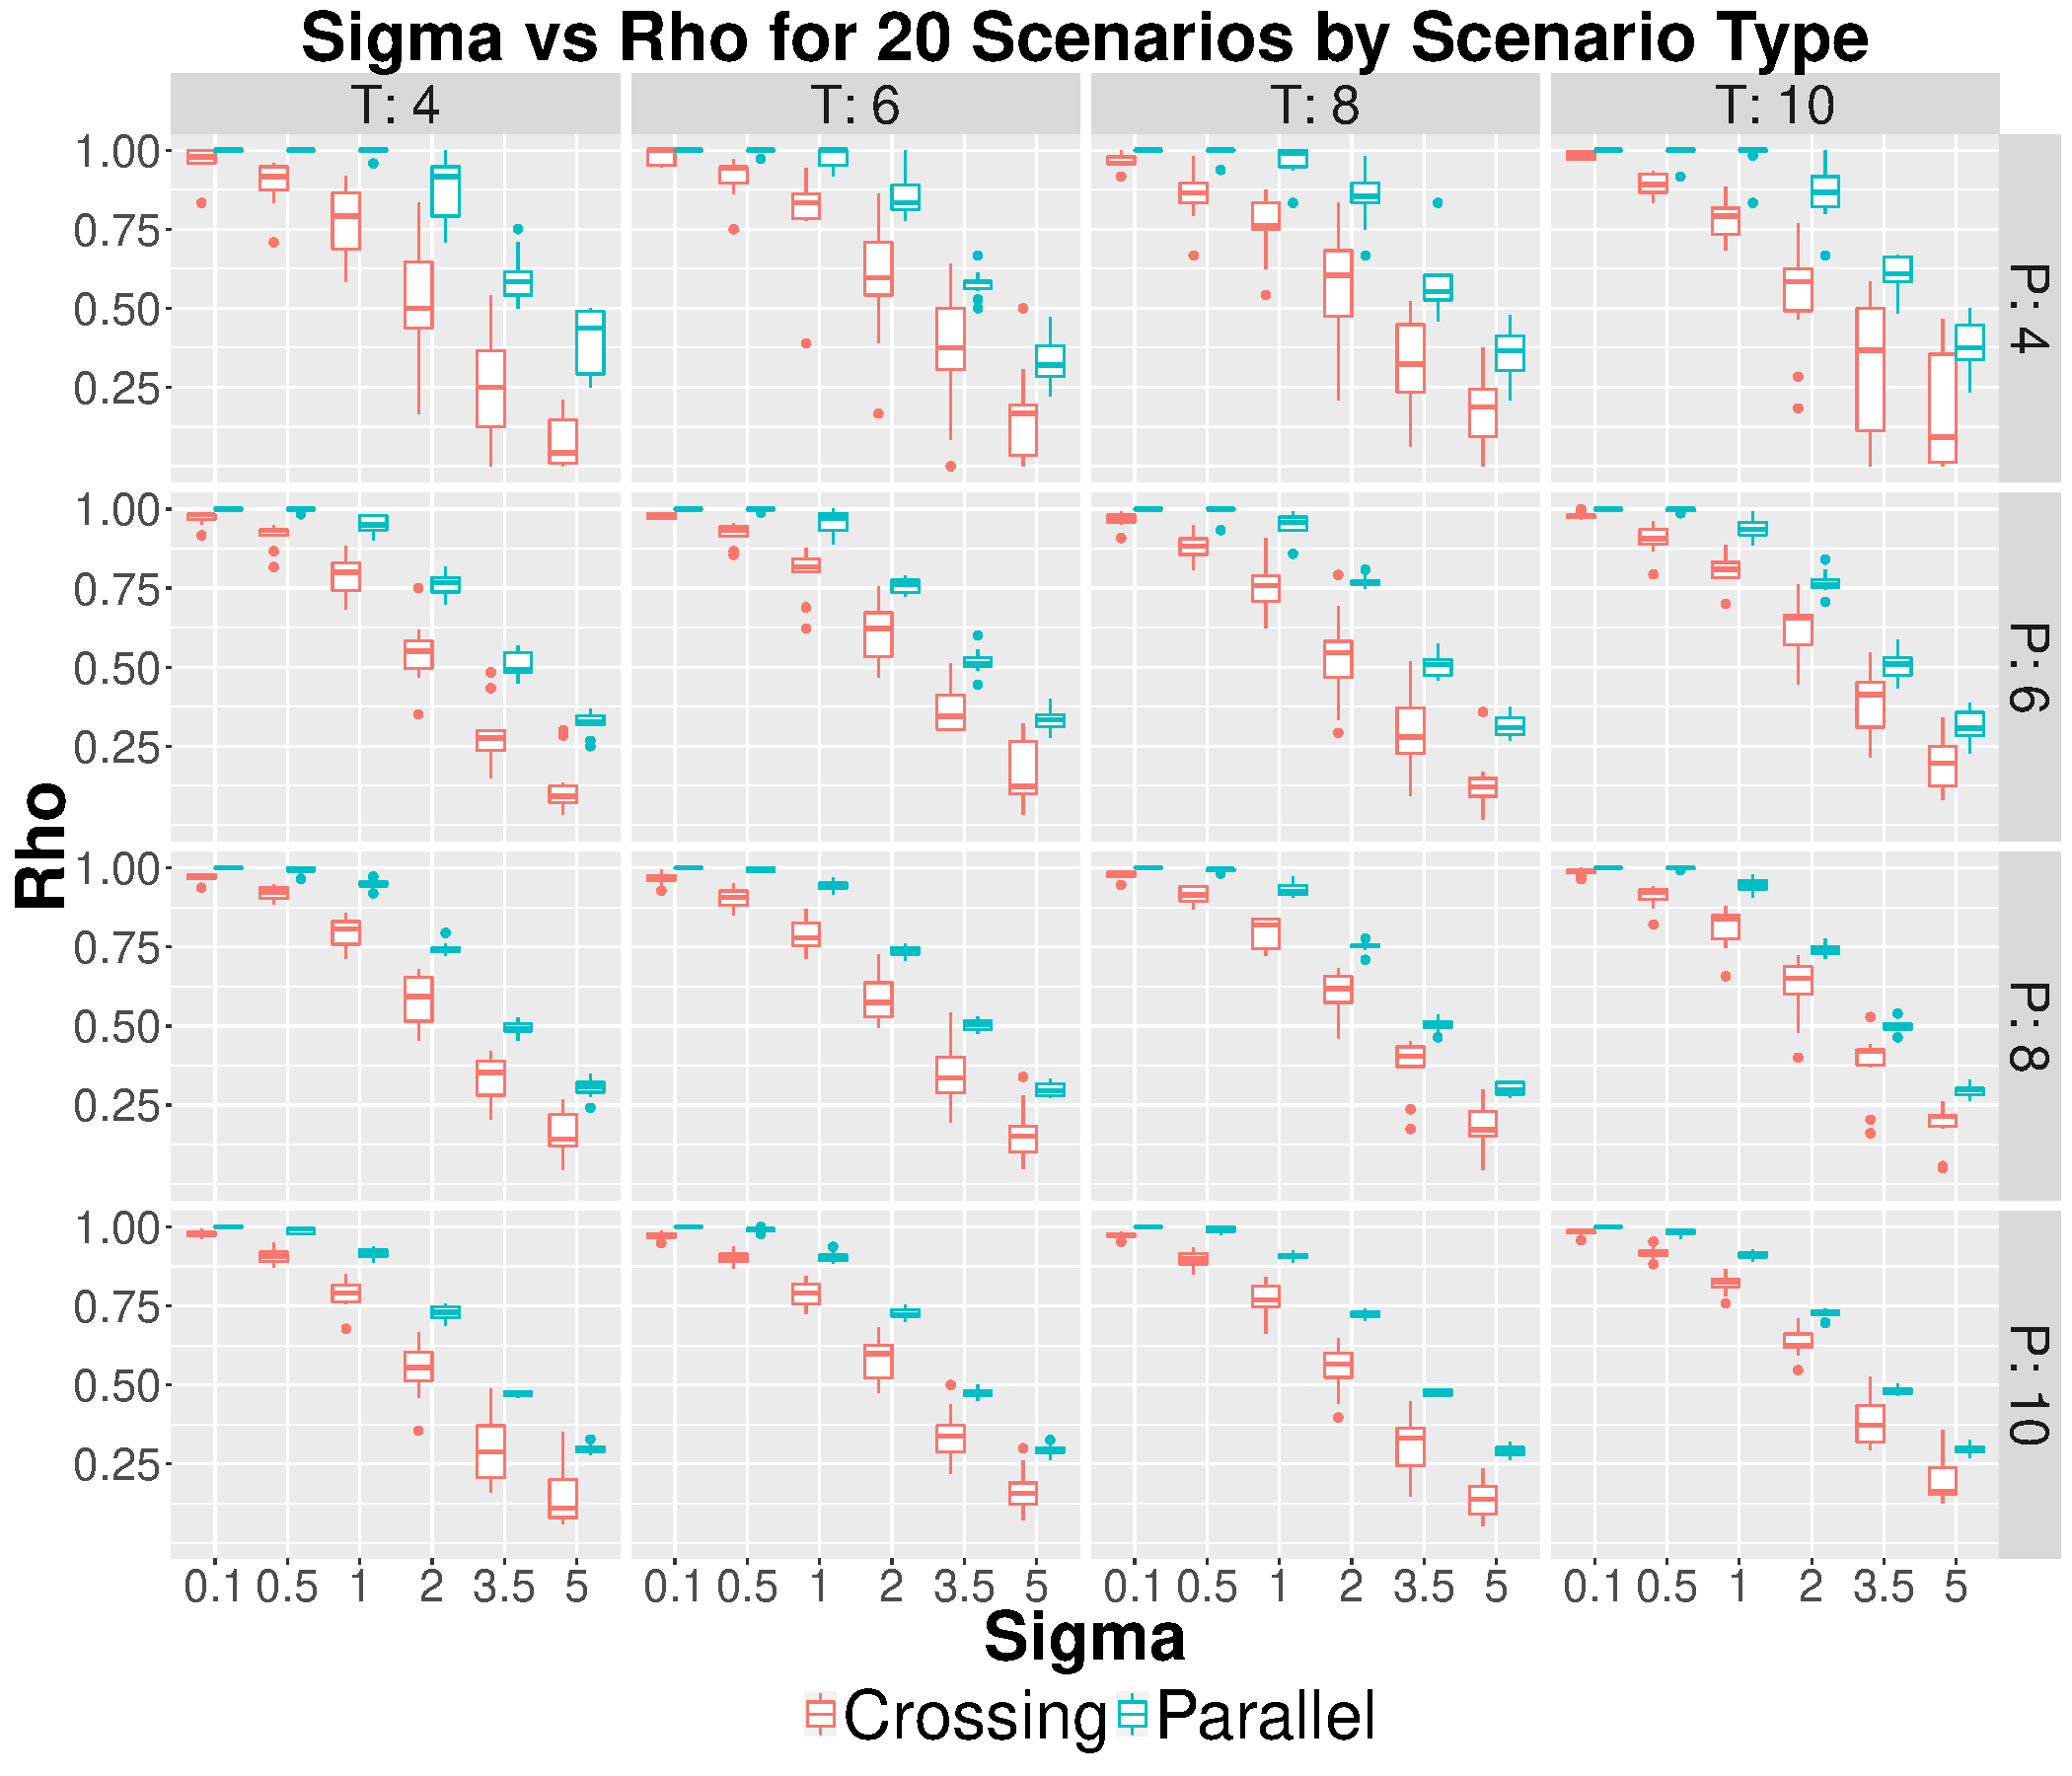
\includegraphics[width=\columnwidth]{../Figures//Sigma_vs_Rho}
    \caption{Relationship between $\sigma$ and $\rho$ summarized by scenario type for all 20 generated scenarios in this experiment.}
    \label{fig:Sigma_vs_Rho}
\end{figure}

Remember that higher values of $\rho$ indicate a lower proportion of detections within very close proximity to one another. We note that the parallel method of scenario generation clearly generates easier scenarios, as measured by $\rho$. This suggests that it may be more difficult to discern correct associations for crossing scenarios than for parallel scenarios. In addition, we can conclude from Figure~\ref{fig:Sigma_vs_Rho} that $\sigma$ and $\rho$ are highly correlated, and the higher $\sigma$ is the lower $\rho$ becomes, which in to be expected from the definition of $\rho$. 

We also note that the range of $\rho$ values corresponding to a single value of $\sigma$ decreases as the number of targets increases. In other words, as the number of targets increases, it becomes more difficult to generate a wider variety of $\rho$ values from a given $\sigma$. For example, for the crossing scenarios with $T=10$ and $\sigma=5$, in the case of four targets the range of $\rho$ is approximately while $[0,0.5]$, while  in the case of ten targets it is limited to $[0.125,0.375]$. Most likely, this is a result of using a fixed state space, as the number of target increases the flexibility of positioning the track decreases.

 Although the variety of difficulty measures decreases as the number of targets increases, the measure $\rho$ still provides a meaningful measure of difficulty for the data association problem. 

\mysubsubsection{The Basic Heuristic Scalability}
We transition to evaluate the scalability of the heuristic run times. Table~\ref{tab:Basic_heuristic_times} summarizes the minimum, mean, and maximum run times of the heuristic for a single starting point, arranged by the number of targets ($P$) and number of scans ($T$). Times are shown in milliseconds. 

\begin{table}[ht]
\centering
\begin{tabular}{cc|ccc}
  \hline
   & & \multicolumn{3}{c}{Basic Heuristic Run Times } \\
   & & \multicolumn{3}{c}{(in milliseconds)}\\
   P & T & $\;\;$Min$\;\;$ & Mean & Max \\ 
  \hline
  \hline
   4 & 4 & 0.07 & 0.10 & 0.18 \\ 
   4 & 6 & 0.18 & 0.24 & 0.38 \\ 
   4 & 8 & 0.34 & 0.45 & 0.62 \\ 
   4 & 10 & 0.58 & 0.76 & 1.02 \\ 
   6 & 4 & 0.11 & 0.15 & 0.25 \\ 
   6 & 6 & 0.31 & 0.39 & 0.58 \\ 
   6 & 8 & 0.64 & 0.81 & 1.05 \\ 
   6 & 10 & 1.24 & 1.56 & 2.02 \\ 
   8 & 4 & 0.14 & 0.19 & 0.30 \\ 
   8 & 6 & 0.46 & 0.57 & 0.86 \\ 
   8 & 8 & 0.95 & 1.24 & 1.58 \\ 
   8 & 10 & 2.07 & 2.53 & 3.37 \\ 
   10 & 4 & 0.19 & 0.25 & 0.41 \\ 
   10 & 6 & 0.63 & 0.80 & 1.03 \\ 
   10 & 8 & 1.44 & 1.84 & 2.44 \\ 
   10 & 10 & 2.96 & 3.73 & 4.56 \\ 
   \hline
\end{tabular}
\caption{Heuristic run times (in milliseconds) for a single starting point.}
\label{tab:Basic_heuristic_times}
\end{table}

Close examination shows that the heuristic scales more efficiently with increases in the number of targets than increases in the number of scans. For example, increasing from four to six scans for four targets increases the computational cost by $140\%$, while increasing from four to six targets for four scans increases the computational cost by $50\%$. The same trend holds true across all targets and scans. Although the heuristic scales more efficiently in $P$ than $T$, the heuristic does not exceed 5 milliseconds in all cases per starting point.

The true scalability of the heuristic is fully realized when we consider the power of parallelization. By running the heuristic on several processors, we can reduce the number of starting points run on each processor, and in turn reduce the total running time. As a result, given enough processors, the heuristic can run several thousand starting points and still find solutions in a fraction of a second. To illustrate this, say that we intend to run 50,000 heuristic starting points for a scenario with six targets and six scans. The average run time for a single starting point of this size is about 0.4 milliseconds. Running all of these starting points in sequence would require approximately 20 seconds of run time, however, those same starting points parallelized onto 100 processors would only require a run time of 0.2 seconds. Thus, the run time of the heuristic can be reduced to meet the efficiency needs of the system, subject only to the limitation of available processors. 

In order to determine the appropriate number of starting points for the heuristic, we examine the MIO objective value of heuristic solutions for various number of starting points, recall that regardless of the number of starting points we will always choose the solution with the best objective function value. For ease of notation, let $f_{H}$ be the MIO objective score of the heuristic solution and $f_{I}$ be the MIO objective score of the ideal solution, which as a reminder is the solution in which the data association problem is exactly correct. We then compute the ratio of $f_{H}/f_{I}$, providing us a normalized measure for comparing the objective score across several scenarios. Figure~\ref{fig:Basic_Heuristic_Objective} plots $f_{H}/f_{I}$ (log scale)  against $\sigma$.
\begin{figure}[ht]
  \centering
  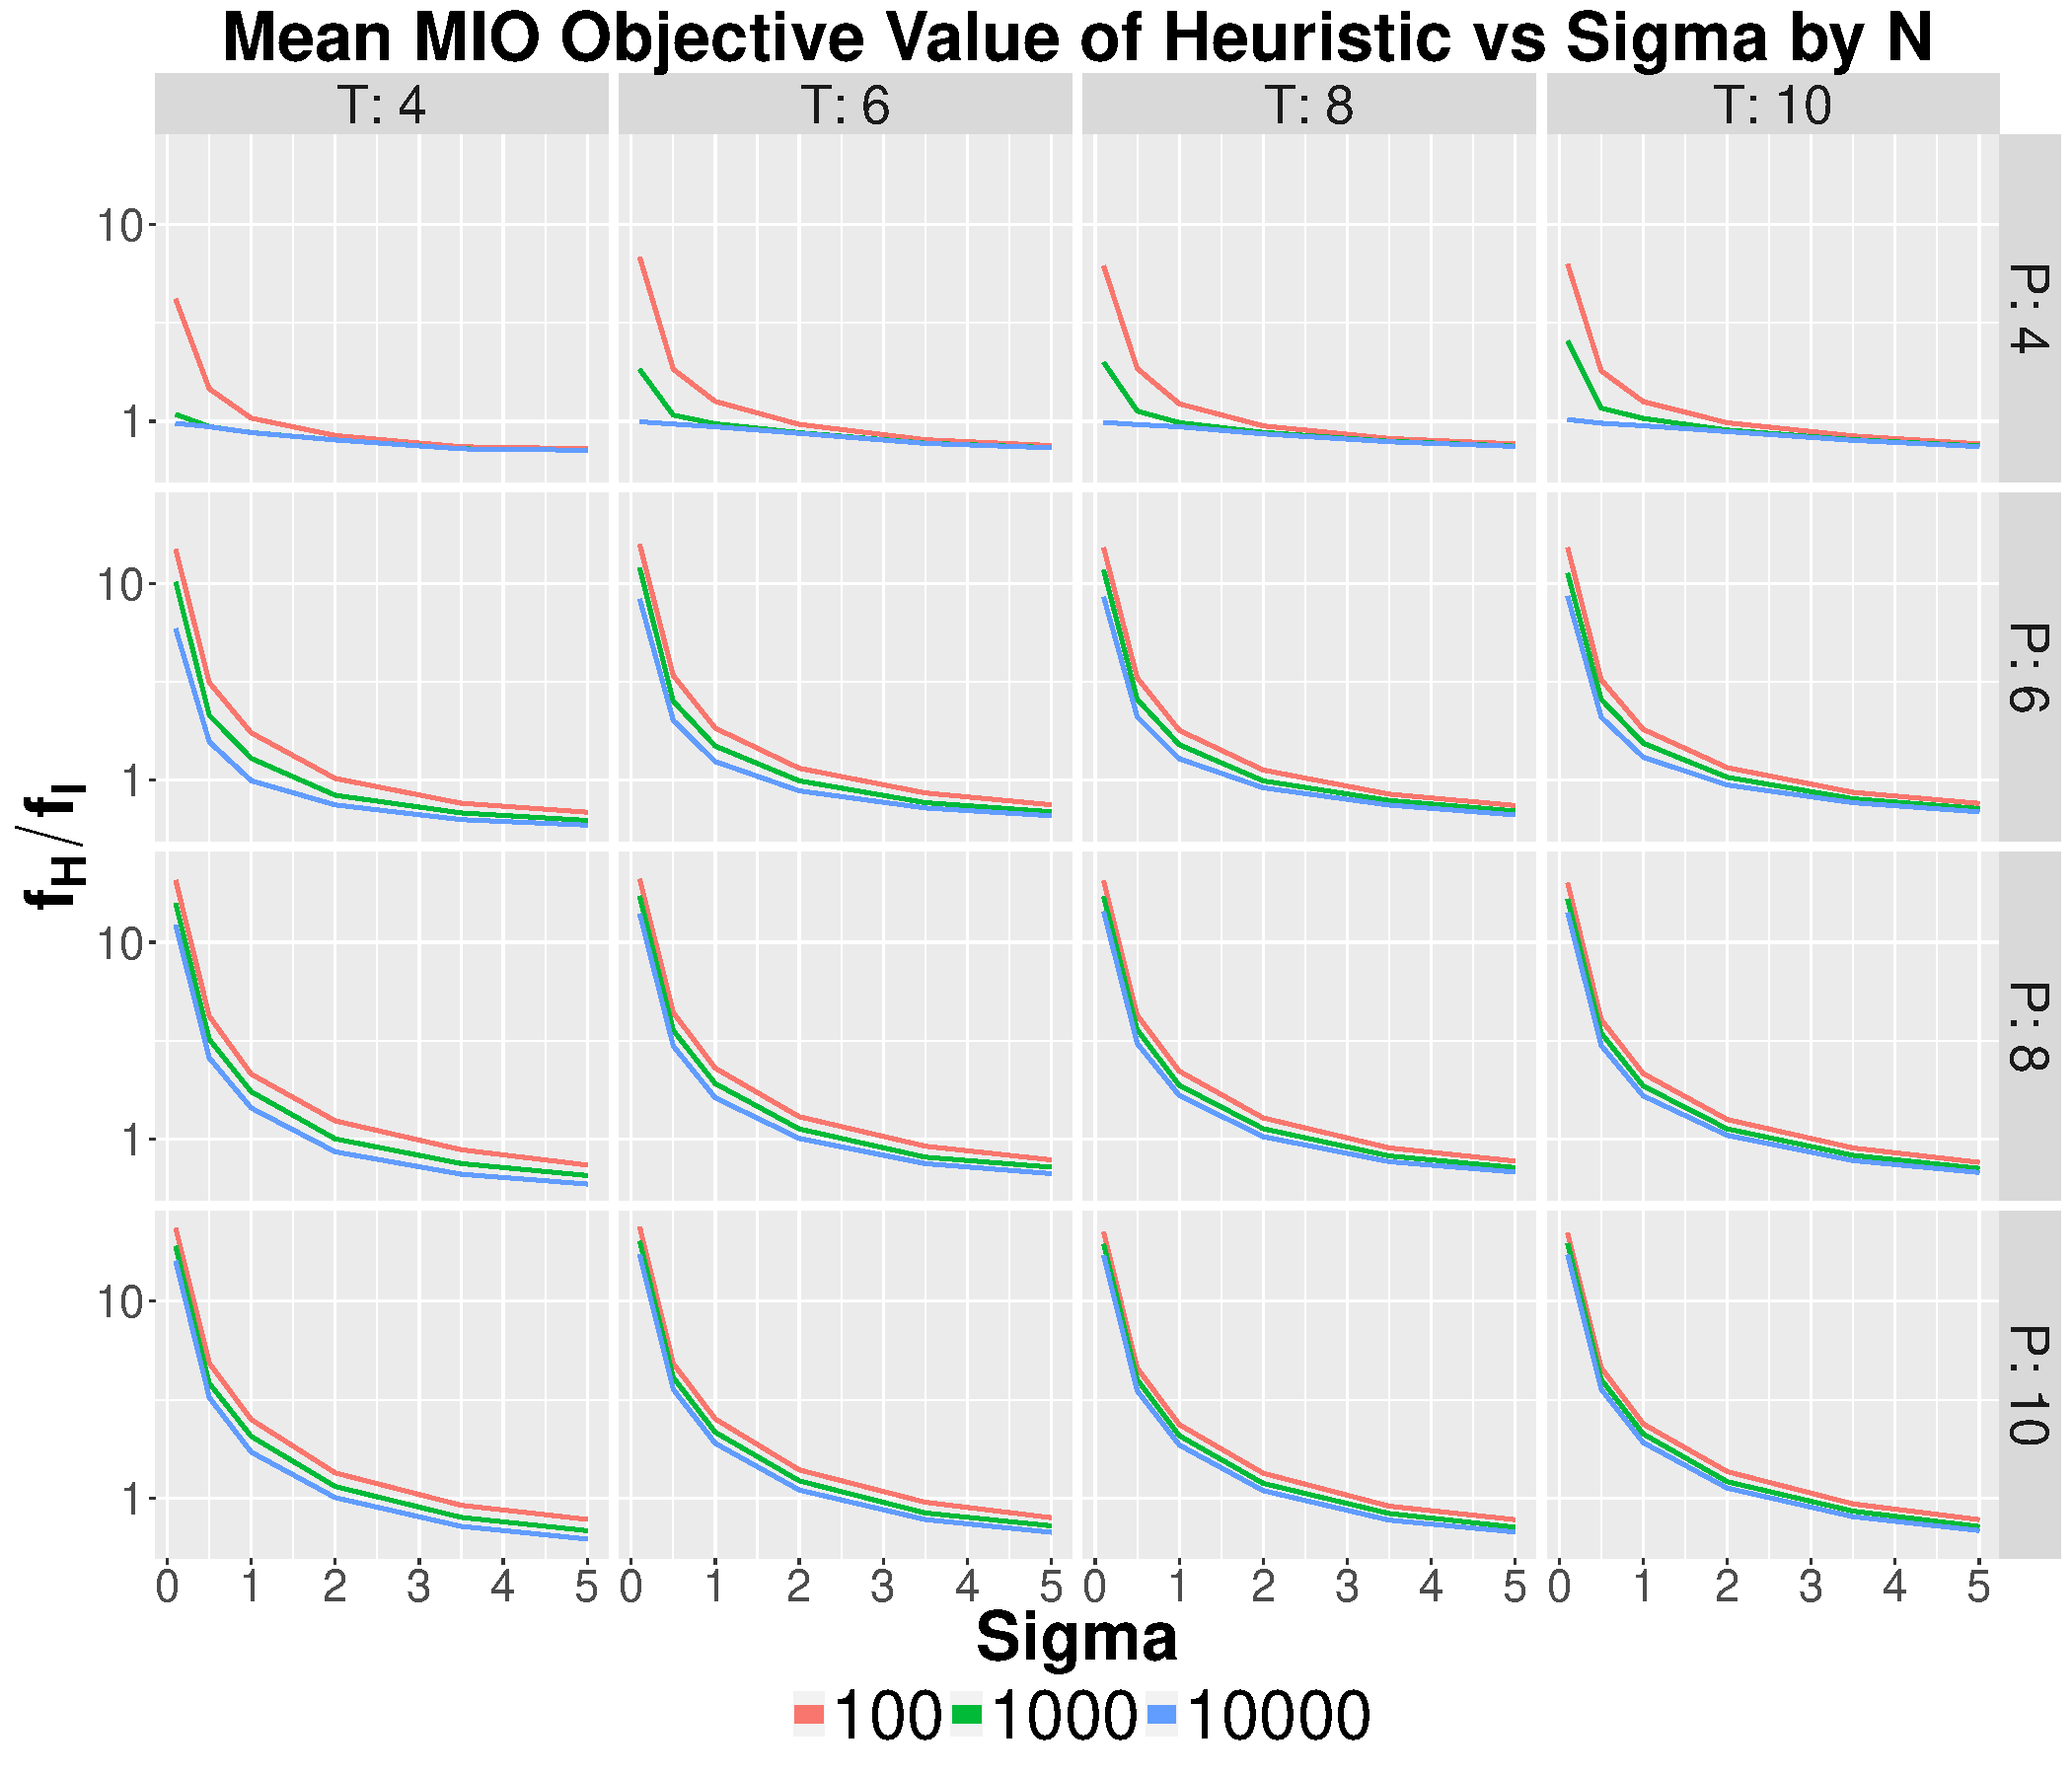
\includegraphics[width=\columnwidth]{../Figures/Basic_Heuristic_Objective}
  \caption{Quality of heuristic solution as compared to the ideal solution's MIO objective value summarized by number of starting points.}
  \label{fig:Basic_Heuristic_Objective}
\end{figure}

In all cases, increasing the number of starting points improves the heuristic solution as compared to the ideal solution. For scenarios of four targets, the improvement is greatest, on the order of about five times improvement from 100 to 10,000 starting points. However, for scenarios with more targets, there is only slight improvement in objective value with increases in the number of starting points. This suggests that in order to improve MIO objective value, the number of necessary starting points increases with $P$, likely due to the exponential increase in combinatorial solutions as the number of targets increases. In any event, we have seen that there is not a significant difference in heuristic performance for the range of $N$ values that we explored. Therefore, for simplification as we move forward in our analysis, we will restrict our discussions of the heuristic to $N=1,000$. 

It is also interesting to note that in some instances the ratio $f_{H}/f_{I}$ falls below the value 1, indicating that the heuristic outperforms the ideal solution, as measured by the objective function. This occurs for higher values of $\sigma$, for example, when the value of $\sigma$ is larger than $2$ regardless of the value of $P$ and $T$. To explain this phenomenon, we must recall that the ideal solution is simply ideal in the sphere of data association, while the MIO objective function serves to provide a measure of solution quality in regards to both data association and trajectory estimation. This seems to suggest that it may be necessary to tradeoff correct data associations in order to improve the trajectory estimation in cases where there is more detection noise. 

With these points in mind we continue our analysis to evaluate solution quality for both the data association problem and trajectory estimation for both the heuristic and MIO solutions.

\mysubsubsection{Data Association}
We shift our focus to analyze the performance of both the basic heuristic and the basic MIO model in regards to the data association problem. Figure~\ref{fig:Basic_Accuracy_Summary} plots the mean accuracy of both solutions against $\rho$, our measure of difficulty for data association. The heuristic shown on the plot was initialized with 1,000 starting points and the MIO model was provided this solution as a warm start. Note that the results for the MIO model do not include the solution at $3T$ seconds, since it exhibited little to no improvement over the MIO solution at $2T$ seconds. The ideal solution, which always achieves an accuracy of 1.0, has also been excluded for the sake of clarity.
\begin{figure}[ht]
  \centering  
  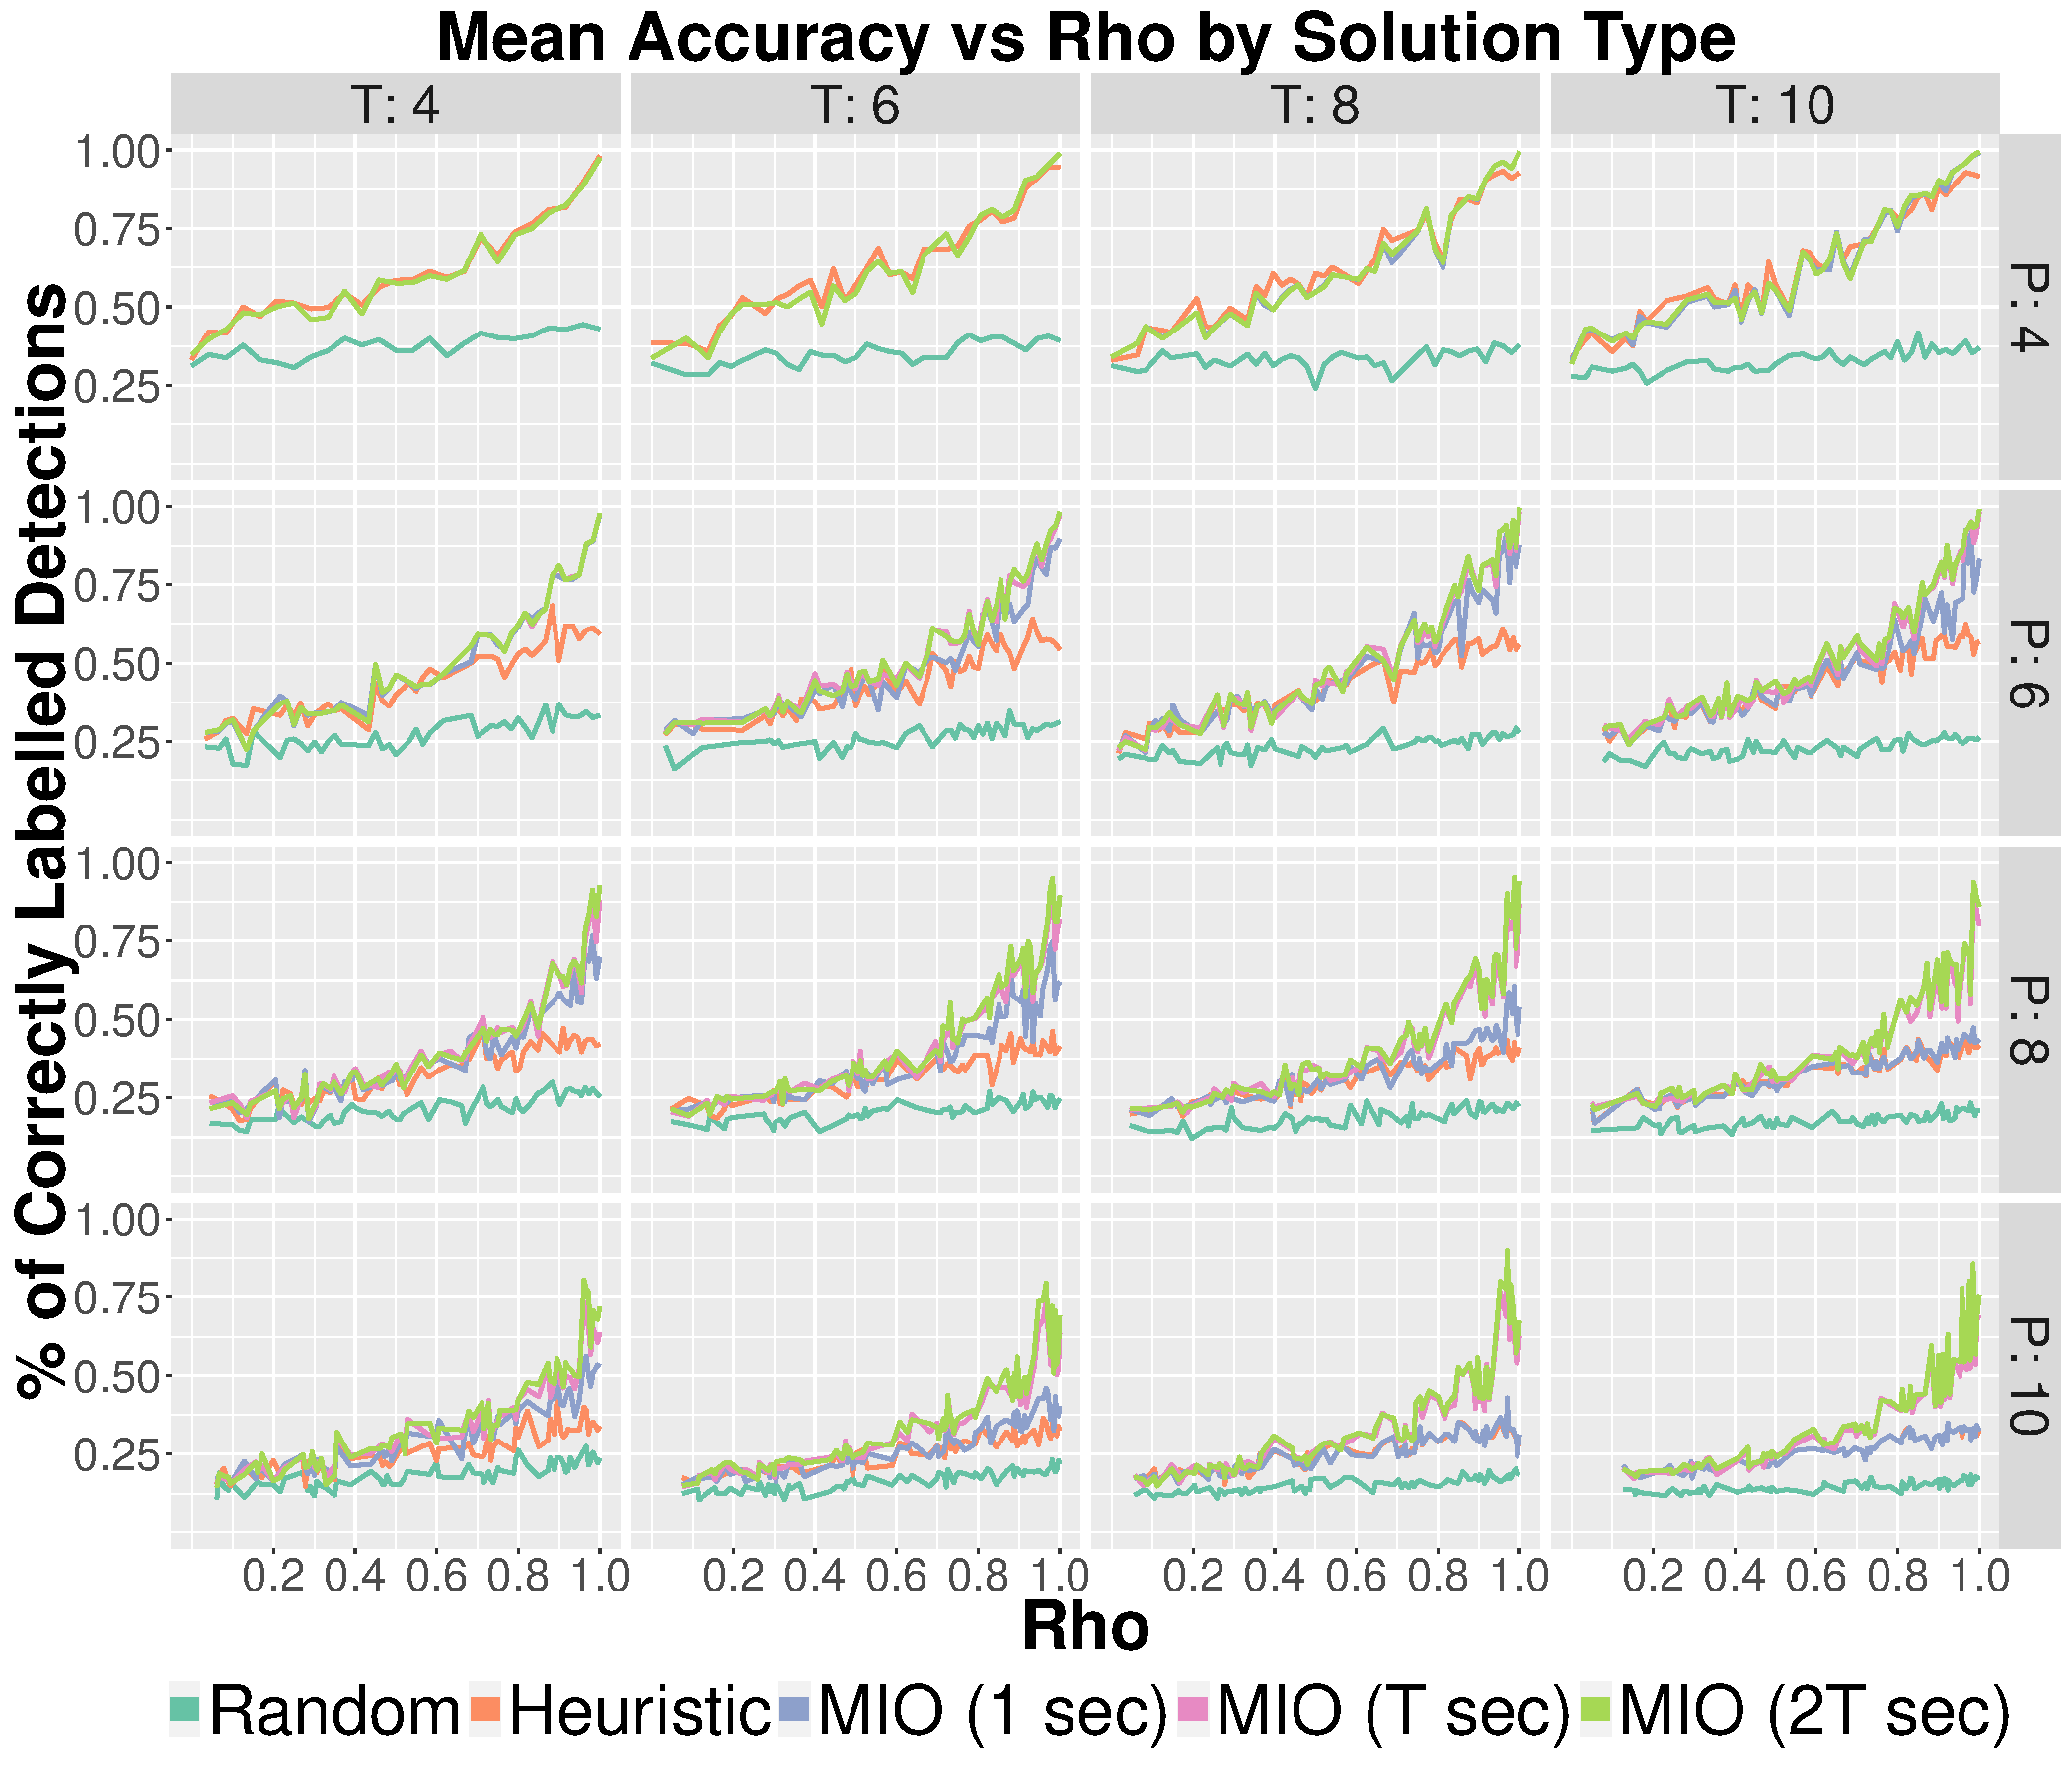
\includegraphics[width=\columnwidth]{../Figures/Basic_Accuracy_Summary}
  \caption{Accuracy of MIO compared against the heuristic and a randomized solution.}
  \label{fig:Basic_Accuracy_Summary}
\end{figure}

Figure~\ref{fig:Basic_Accuracy_Summary} shows that the quality of the associations found by both the heuristic and the MIO are indeed highly correlated with the scenario complexity parameter $\rho$, and the number of correct association in both increase as $\rho$ reaches $1$. Where for 4 and 6 targets the association is extremely close or exactly the ideal association, when $\rho$ is equal to $1$. In contrast the random association is unaffected by the value of $\rho$ and it accuracy is always lower than the heuristic accuracy. 

In general, it seems that running the MIO for $T$ or less seconds is optimal, since longer running times do not improve the accuracy attained. Specifically, for scenarios of four targets, the best accuracy is reached after $1$ second, while for scenarios of eight and ten targets, the best accuracy is reached after $T$ seconds. 

In scenarios of all sizes, the heuristic improves over the random solution, suggesting that the heuristic finds good quality solutions. In fact, for scenarios of four targets, the heuristic performs equally as well as the MIO model across all numbers of scans. While for scenarios with more targets, the heuristic does not perform as well as the MIO, it still provides good solutions from which the MIO benefits. In particular, for scenarios with eight and ten targets the MIO after $T$ seconds provides about a $30\%$ improvement over the heuristic solution. Moreover, it seems that as the number of targets increases the accuracy deteriorates, due to the added combinatorial difficulty of the association problem. 

Both algorithms appear to scale well with increases in the number of scans. In fact, the accuracy of MIO solutions appear to improve as the number of scans increases. For example, in the case of ten targets, the accuracy of the MIO after $T$ (or $2T$) seconds is higher for eight and ten scans than for four and six scans, especially for high values of $\rho$. This could suggest that the MIO benefits from additional scans, likely a result of the additional information gained from increasing the number of detections. For a fixed number of targets, there appears to be no change in heuristic solution quality as the number of scans changes. 

\mysubsubsection{Trajectory Estimation}
Next, we evaluate the performance of the basic heuristic and MIO through the lens of trajectory estimation. As discussed previously, we are interested in comparing $\delta$, our proxy for ground track error, against $\sigma$, our measure of difficulty for trajectory estimation, in order to analyze performance of in the sphere of estimation. Figure~\ref{Fig:Basic_Delta_Summary} plots $\sigma$ against $\delta$ for each of the previous solution types in addition to the ideal solution. 
\begin{figure}[ht]
  \centering
  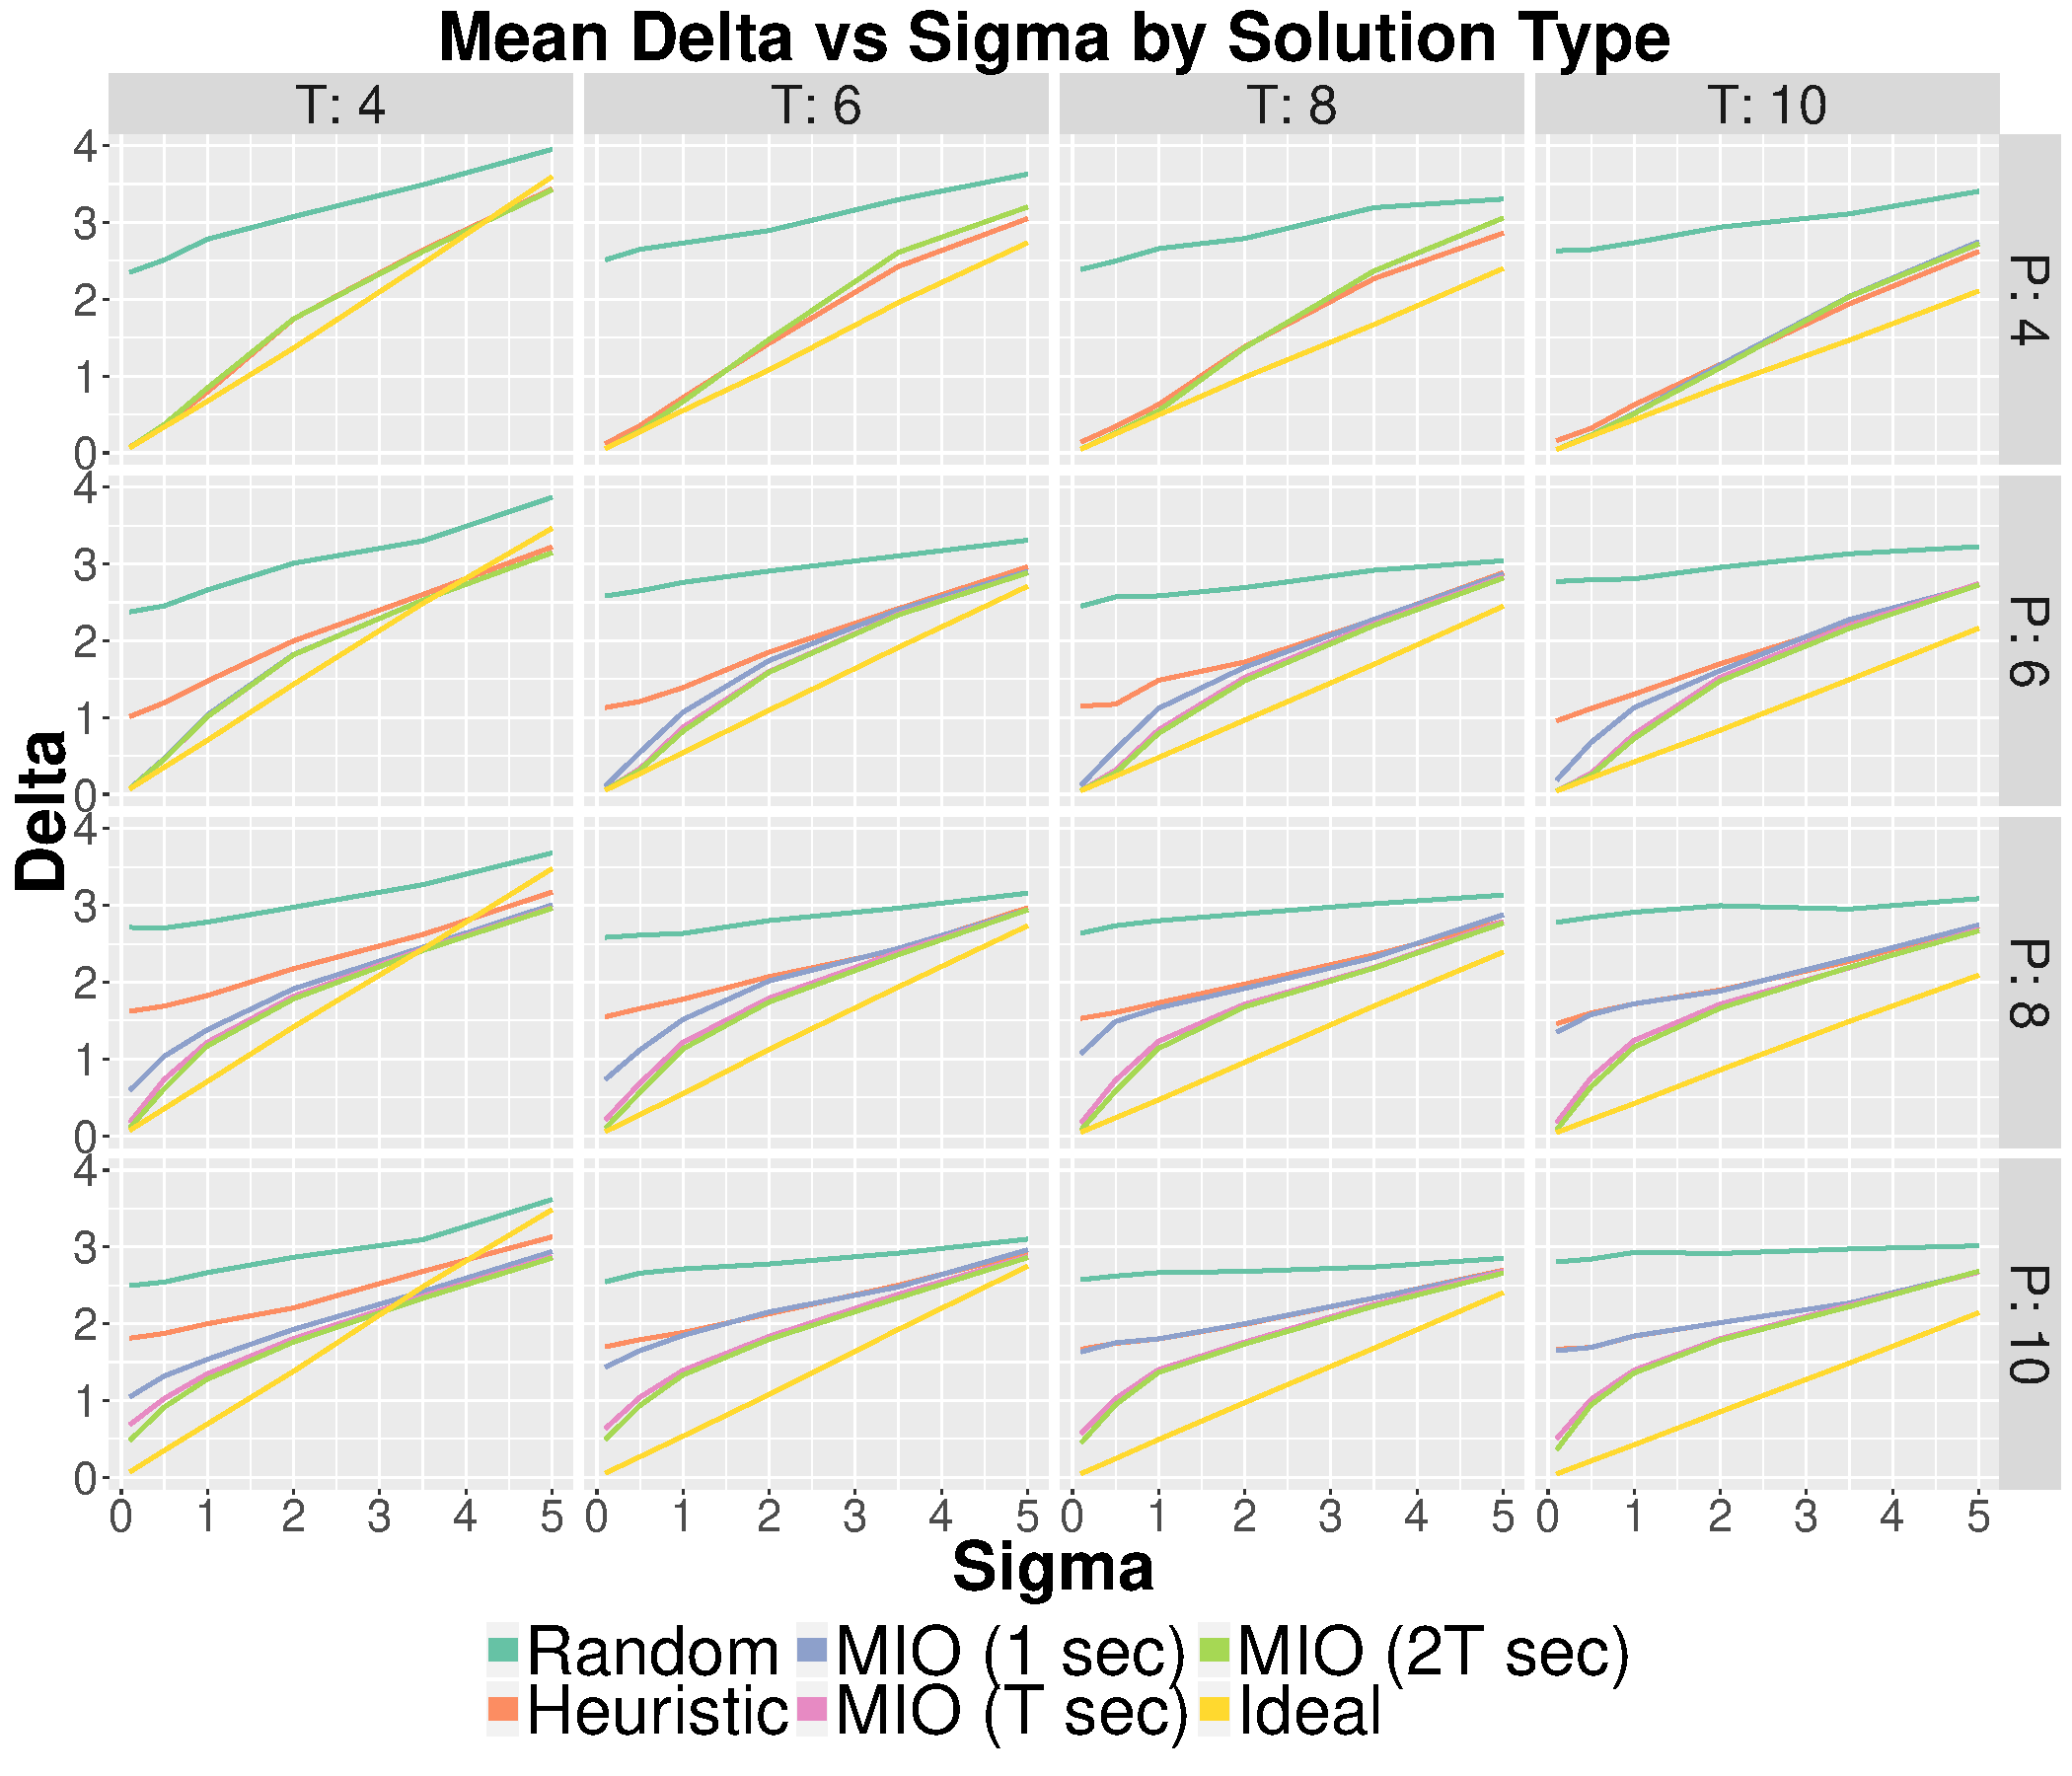
\includegraphics[width=\columnwidth]{../Figures/Basic_Delta_Summary}
  \caption{Trajectory estimation performance}
  \label{Fig:Basic_Delta_Summary}
\end{figure}

Remember that lower values of delta correspond to trajectory estimations that are closer to that of the true ground track. We note that as $\sigma$ approaches zero, both the heuristic and MIO trajectory estimates approach the trajectory estimates of the ideal solution, suggesting that both algorithms find very high quality trajectory estimates in these cases. Similar to the data association, it can be seen that the best estimates are reached after $1$ second for scenarios with four targets and after $T$ seconds for all other scenarios.

The heuristic and MIO outperform the ideal solution in scenarios with only four scans and high values of $\sigma$. However, the algorithms do not outperform the ideal solution for larger numbers of scans. Moreover, the ideal solution estimation changes linearly with sigma, but the slope of this linear dependence decreases as the number of scans increases. This suggests that as the number of scans approaches infinity, the estimated trajectories given by the ideal association will converge to the true ground tracks, even for large sigma values. This is also true for the MIO and heuristic solutions but to a lesser extent, which can be seen by the fact they move further away from the ideal solution when the number of scan increase, showing the tradeoff between added information and computational complexity.

We that the MIO and heuristic solutions estimation error have a bounded distance from the ideal one, and is always outperforms the random solution even for large values of $\sigma$. Which implies that though we do not necessarily get the optimal solution, the guiding objective prevents us from finding solution which are very poor. In particular, the gap between the ideal estimation error and the heuristic/MIO estimation error remains relatively constant across all values of $P$ for a fixed number of scans. 

\mysubsubsection{Summary of Results}
We have shown that in the case of no detection ambiguity
\begin{itemize}
\item The heuristic is highly scalable, and we can finds good quality solutions in fractions of a second using parallelization. 
\item Using these solutions as a warm start, the MIO achieves high quality solutions to both the data association and trajectory estimation measures after $T$ or fewer seconds. 
\item The MIO is scalable with respect to increases in both the number of targets and scans. We have also identified that there exists a tradeoff between making correct data associations and improved trajectory estimation, particularly in cases of high signal to noise ratios. 
\item Increasing the number of scans, while adding computational complexity to the model, helps to obtain better solutions. 
\end{itemize}
With these points in mind, we advance to discussing the case of scenarios with detection ambiguity. 

\mysubsection{Scenarios with Detection Ambiguity}
Here we extend our discussion to analyze the performance of our methods on scenarios with detection ambiguity. We first summarize our experimental methods before discussing performance of both the robust heuristic and the robust MIO in the spheres of both the data association and trajectory estimation problems.

This experiment serves as an extension of the basic one, in order to test the performance of our algorithms under detection ambiguity. We use the same scenarios generated from the basic experiment, however due to the additional difficulty inherent with detection ambiguity, we limit the range of signal noise to $\sigma \in \{0.1,0.5,1.0,2.0\}$, choosing to exclude the extreme cases of signal noise. In addition, we simulate both missed detections and false alarms. A detection is removed with probability, $\gamma$, and we consider $\gamma \in \{0.2,0.15,0.1,0.05\}$. We do not allow empty scans. For each scan, we generate false alarms according to a poisson distribution with parameter, $\lambda$, and false alarm locations are randomly selected uniformly within the state space. We consider $\lambda \in \{0.1,0.5,0.1,2.0\}$. The false alarms are then added to $\mathcal{X}_{t}$ and the detection order of $\mathcal{X}_{t}$ is randomly shuffled in the same manner as the first experiment. 

Once the data has been generated, we follow the same sequence of steps as outlined for the basic experiment, running the heuristic first and then feeding the solution into the MIO as a warm start. Note that the heuristic is only initialized with 1,000 starting points, as determined from the results of the basic experiment. Once again, the optimization process was set to terminate after $2T$ seconds, with solutions collected at intervals of $\{1,T,2T\}$ seconds. Prior to the running of this experiment, we performed a mini experiment and used the results to tune the penalties $\theta$ and $\phi$, a summary of the exact penalties used along with an explanation of the insight behind them, can be found in Appendix~\ref{app:Penalty_Appendix}. An important thing to note with regard to the penalties is that while the estimation error and the number of missed detections are highly correlated with the number of targets, the number of false alarms are not, and so the penalty $\theta$ is set to be linearly dependent on the number of estimated targets. In order to decide on the final estimated target number, we compared the average performance, i.e., the MIO objective function divided by the estimated number of targets, and chose the best one. 

\mysubsubsection{Robust Heuristic} Table~\ref{tab:Robust_heuristic_times} summarizes the minimum, mean, and maximum run times of the heuristic from the robust heuristic for a single starting point, arranged by the number of estimated targets ($P_{\text{est}}$) and number of scans ($T$). Times are shown in milliseconds. 
\begin{table}[ht]
\centering
\begin{tabular}{cc|ccc}
  \hline
   & & \multicolumn{3}{c}{Robust Heuristic Run Times} \\
   & & \multicolumn{3}{c}{(in milliseconds)}\\
   $ P_{\text{estimated}}$ & T & $\;\;$Min$\;\;$ & Mean & Max \\ 
  \hline
  \hline
  2 & 4 & 0.15 & 0.23 & 0.41 \\ 
  2 & 6 & 0.42 & 0.56 & 0.93 \\ 
  2 & 8 & 0.77 & 1.04 & 2.24 \\ 
  2 & 10 & 1.27 & 1.73 & 3.07 \\ 
  4 & 4 & 0.15 & 0.34 & 1.04 \\ 
  4 & 6 & 0.50 & 0.94 & 2.69 \\ 
  4 & 8 & 1.09 & 1.88 & 3.87 \\ 
  4 & 10 & 2.12 & 3.25 & 7.20 \\ 
  6 & 4 & 0.14 & 0.42 & 0.96 \\ 
  6 & 6 & 0.57 & 1.29 & 4.45 \\ 
  6 & 8 & 1.33 & 2.66 & 5.82 \\ 
  6 & 10 & 2.53 & 4.61 & 9.4 \\ 
  8 & 4 & 0.16 & 0.50 & 1.10 \\ 
  8 & 6 & 0.60 & 1.59 & 3.46 \\ 
  8 & 8 & 1.38 & 3.37 & 6.87 \\ 
  8 & 10 & 2.63 & 5.84 & 12.40 \\ 
  10 & 4 & 0.18 & 0.55 & 1.10 \\ 
  10 & 6 & 0.72 & 1.82 & 3.98 \\ 
  10 & 8 & 1.53 & 3.96 & 8.18 \\ 
  10 & 10 & 3.42 & 6.93 & 13.93 \\ 
  12 & 4 & 0.16 & 0.56 & 0.99 \\ 
  12 & 6 & 0.99 & 1.95 & 3.96 \\ 
  12 & 8 & 1.74 & 4.33 & 8.69 \\ 
  12 & 10 & 3.40 & 7.71 & 15.10 \\ 
   \hline
\end{tabular}
\caption{Robust heuristic run times (in milliseconds) for a single starting point.}
\label{tab:Robust_heuristic_times}
\end{table}

As expected, the robust heuristic requires longer run times than the basic heuristic, due to the increase in combinatorial solutions to the assignment problem. Comparing Table~\ref{tab:Basic_heuristic_times} and Table~\ref{tab:Robust_heuristic_times} we see that robust run times for four estimated targets are roughly four times longer than the corresponding run times in the basic heuristic for a fixed number of scans. However, the magnitude of this effect appears to decay as the number of targets increases. For example, in the case of eight targets, the robust heuristic times are only about twice that of the basic heuristic. This suggests that the robust heuristic still scales well with increases in the number of targets. It is also important to note that the run time variance in the robust case is much wider than the one for the basic case. However, parallelization might somewhat relieve this issue enabling the actual runtime to e closer to the average.

As exhibited by the basic heuristic, the scalability with regard to $P_{\text{est}}$ is better than with regard to $T$. For example, increasing from eight to ten scans for eight targets increases the computational cost by $140\%$, while increasing from eight to ten targets for eight scans increases the computational cost by $50\%$. Here, we must remind the reader, that for each scenario we actually have to check several $P_{\text{est}}$ values, which requires additional processing time and parallelization. In our simulations, we found that the range of possible $P_{\text{est}}$ values was generally limited to six values. 

\mysubsubsection{Number of Targets}
In the case of detection ambiguity, in order to correctly estimate the trajectories we must first correctly estimate the number of targets, consequently making this task extremely important. Therefore, we begin our analysis of detection ambiguity by evaluating the difference between the true and estimated number of targets. Explicitly, we define:
\begin{align}
	P_{\text{diff}} = P_{\text{true}} - P_{\text{est}},
\end{align}
where $P_{\text{est}}$ is the number of estimated targets and $ P_{\text{true}}$ is the number of true targets. Note that $P_{\text{diff}} = 0$ indicates that we have correctly estimated the number of targets. When $P_{\text{diff}} < 0$, we have overestimated the number of targets, whereas when $P_{\text{diff}} > 0$, we have underestimated the number of targets. Figure~\ref{fig:Robust_4_8_Histogram} plots the distribution of $P_{\text{diff}}$ for scenarios with four targets and eight scans, and for comparison, Figure~\ref{fig:Robust_8_8_Histogram} plots the same result for scenarios of eight targets and eight time scans. 
\begin{figure}[ht]
  \centering
  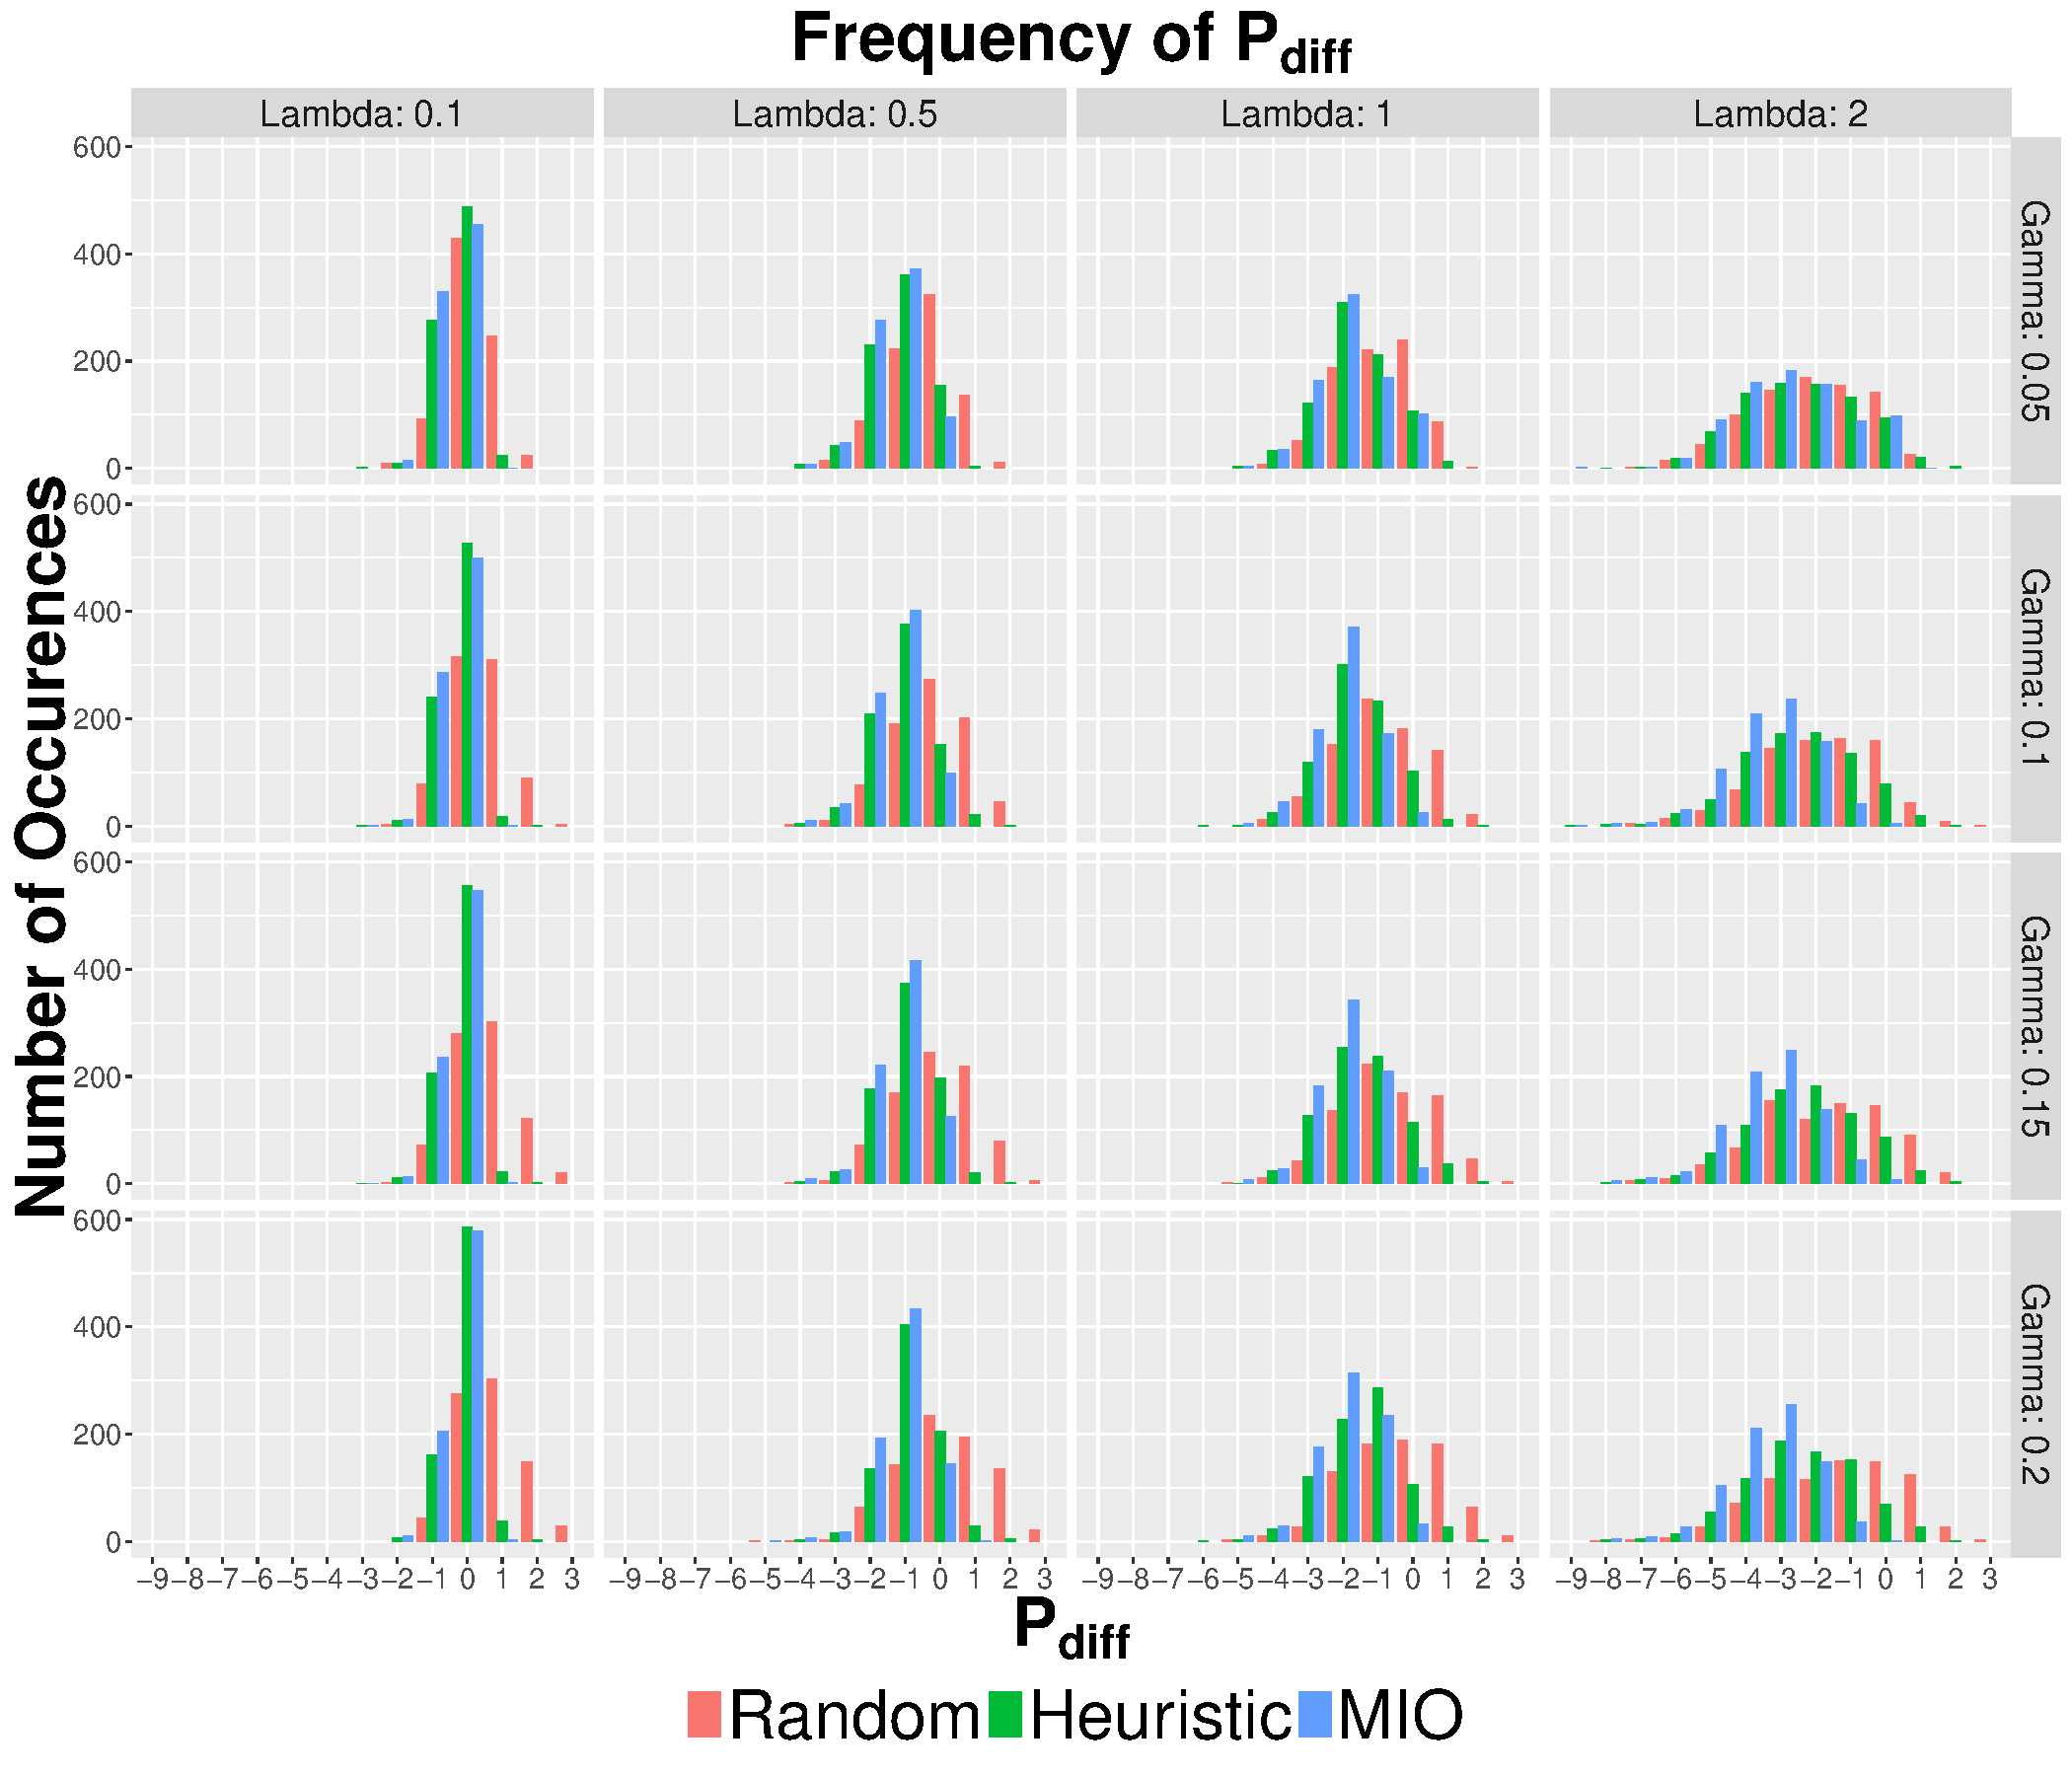
\includegraphics[width=\columnwidth]{../Figures/4_8_Histogram}
  \caption{Distribution of the difference in true and estimated number of targets for scenarios with 4 targets and 8 scans, arranged by $\gamma$ and $\lambda$.}
  \label{fig:Robust_4_8_Histogram}
\end{figure}
\begin{figure}[ht]
  \centering
  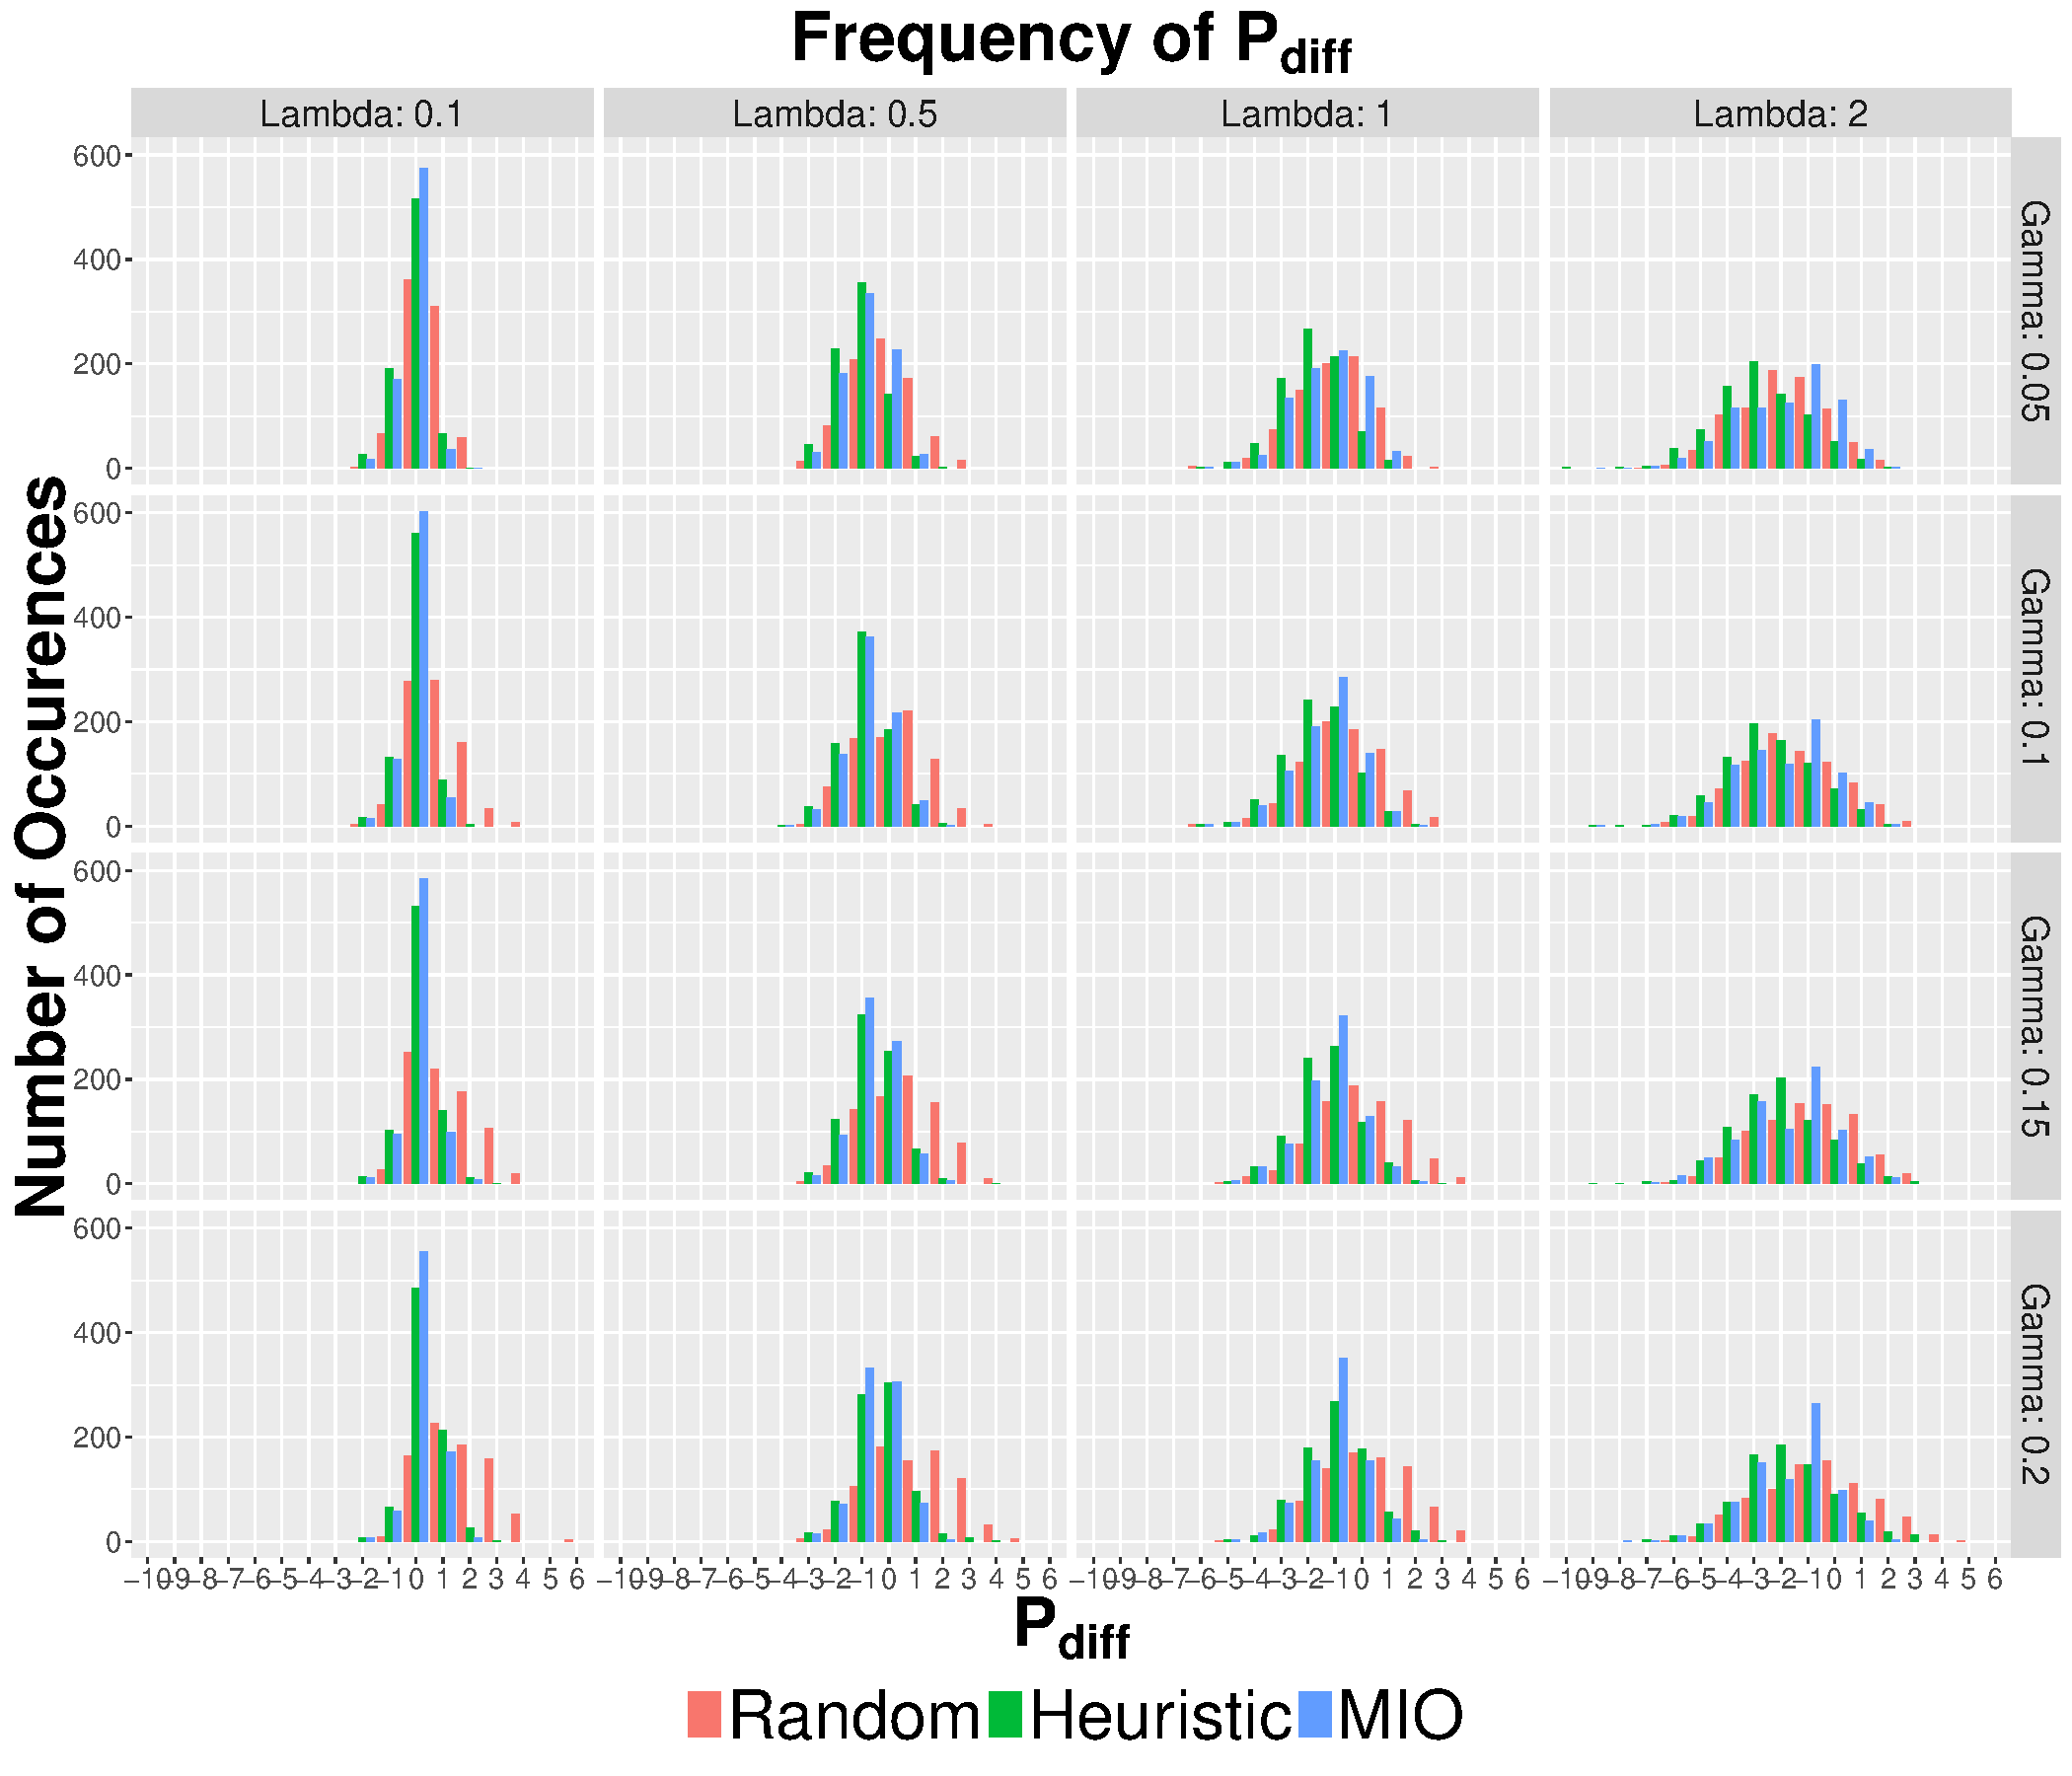
\includegraphics[width=\columnwidth]{../Figures/8_8_Histogram}
  \caption{Distribution of the difference in true and estimated number of targets for scenarios with 8 targets and 8 scans, arranged by $\gamma$ and $\lambda$.}
  \label{fig:Robust_8_8_Histogram}
\end{figure}

We see that both the robust heuristic and the robust MIO estimate the number of targets correctly a very high proportion of the time in both scenario sizes when $\lambda = 0.1$. As $\lambda$ increases, we see a tendency to overestimate the number of targets. This trend appears to be more prominent in Figure~\ref{fig:Robust_4_8_Histogram}, meaning that the scenario with four targets has a higher tendency to overestimate for large values of $\lambda$ than the scenario with eight targets. Further examination shows that both solutions have slightly fewer false alarms than the ideal solution for scenarios with eight targets, and this effect is slightly more exaggerated for the scenarios with four targets. This suggest that $\theta$ was set too high, or alternatively that, the missed detection penalty $\phi$ was too low, which is also supported by the fact that both algorithms identified too many missed detections. Altogether, this suggests that the algorithms likely took a preference to create additional trajectories misclassifying the false alarms as detections for these targets as well as assigning them many missed detections, ultimately resulting in a tendency to overestimate the number of targets. A finer tuning of $\theta$ and $\phi$ can resolve this problem, however, we find it difficult to tune these parameters for higher levels of the false alarm rate $\lambda$, which explains why this over estimation is worse as $\lambda$ increases. Moreover, it is difficult to tune the parameters to obtains the same tendencies for different number of targets, however, we do not know the true  number of targets, which leads us to believe that more sophisticated penalty functions are needed to neutralize this difference.

\mysubsubsection{Data Association}
Knowing that we tend to overestimate the number of targets with the given penalties, we move on in our analysis to measuring the accuracy of our robust approaches. Figures~\ref{fig:Robust_4_8_Accuracy} and~\ref{fig:Robust_8_8_Accuracy} plot accuracy against the difficulty metric, $\rho$, for scenarios of four and eight targets, respectively. Both scenarios have eight scans and both figures have been arranged by $\gamma$ and $\lambda$.
\begin{figure}[ht]
  \centering
  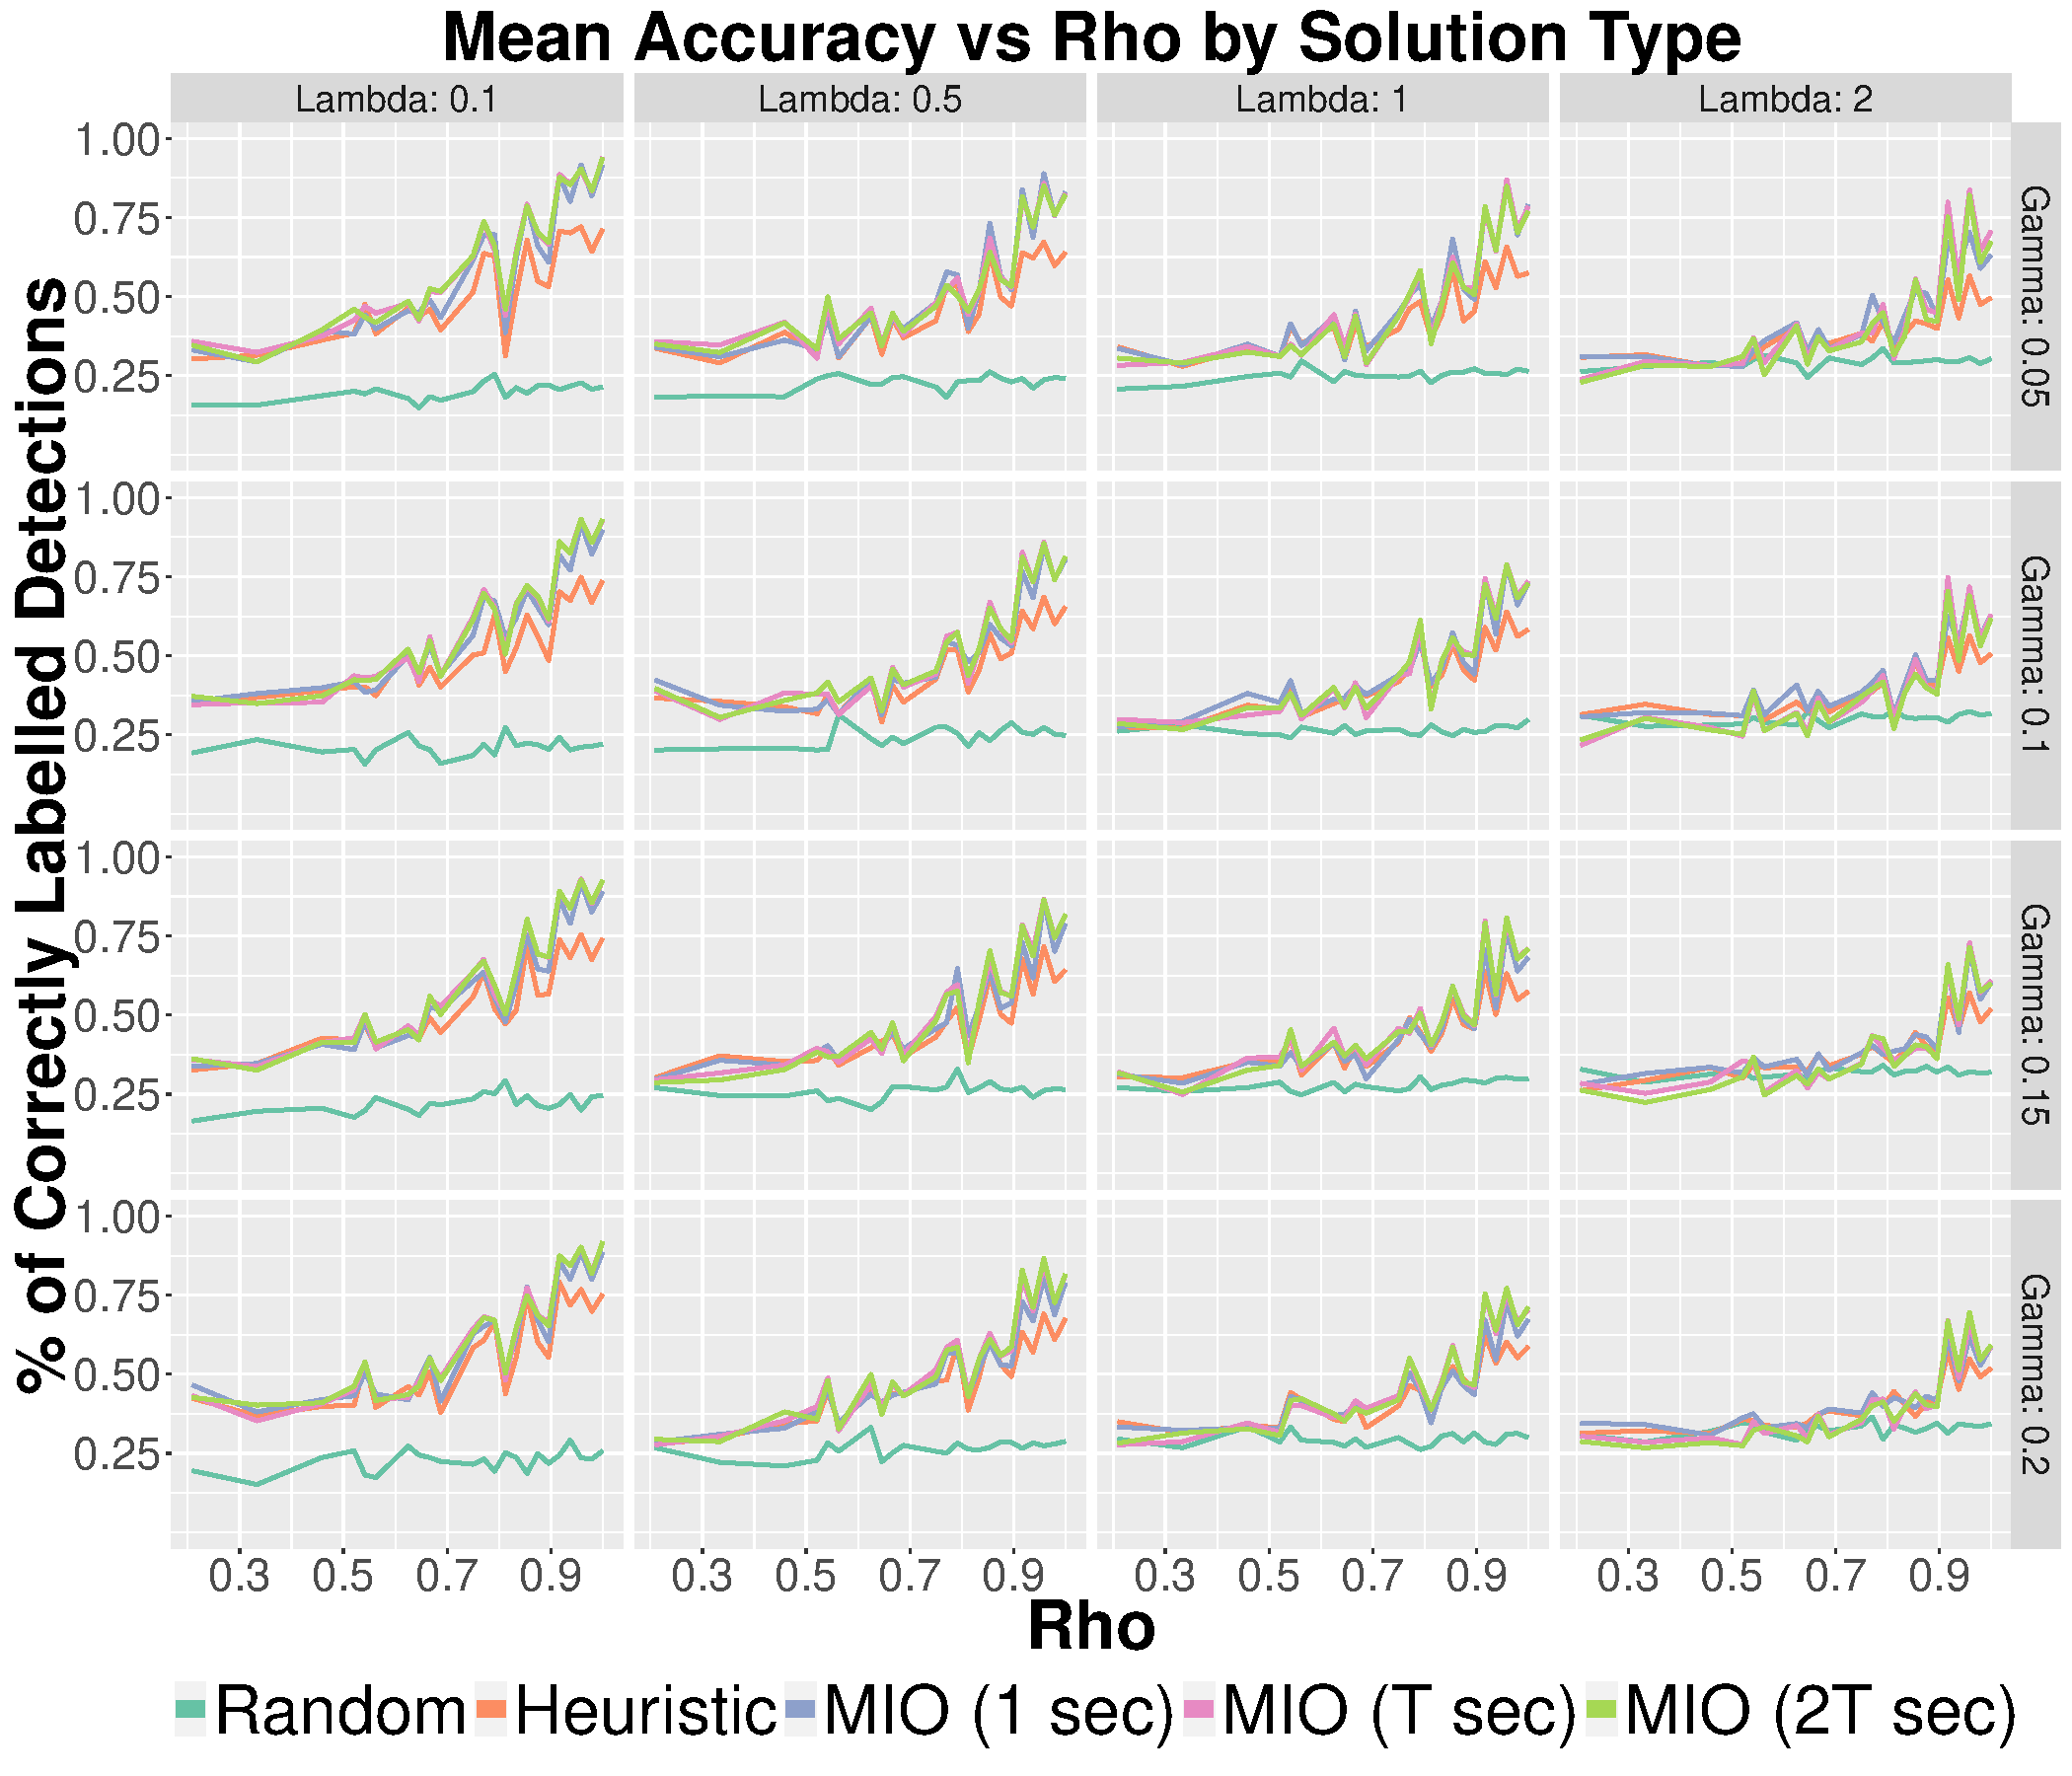
\includegraphics[width=\columnwidth]{../Figures/4_8_Accuracy}
  \caption{Accuracy of robust heuristic and MIO as compared to random solutions for scenarios of 4 targets and 8 scans, arranged by $\gamma$ and $\lambda$.}
  \label{fig:Robust_4_8_Accuracy}
\end{figure}
\begin{figure}[ht]
  \centering
  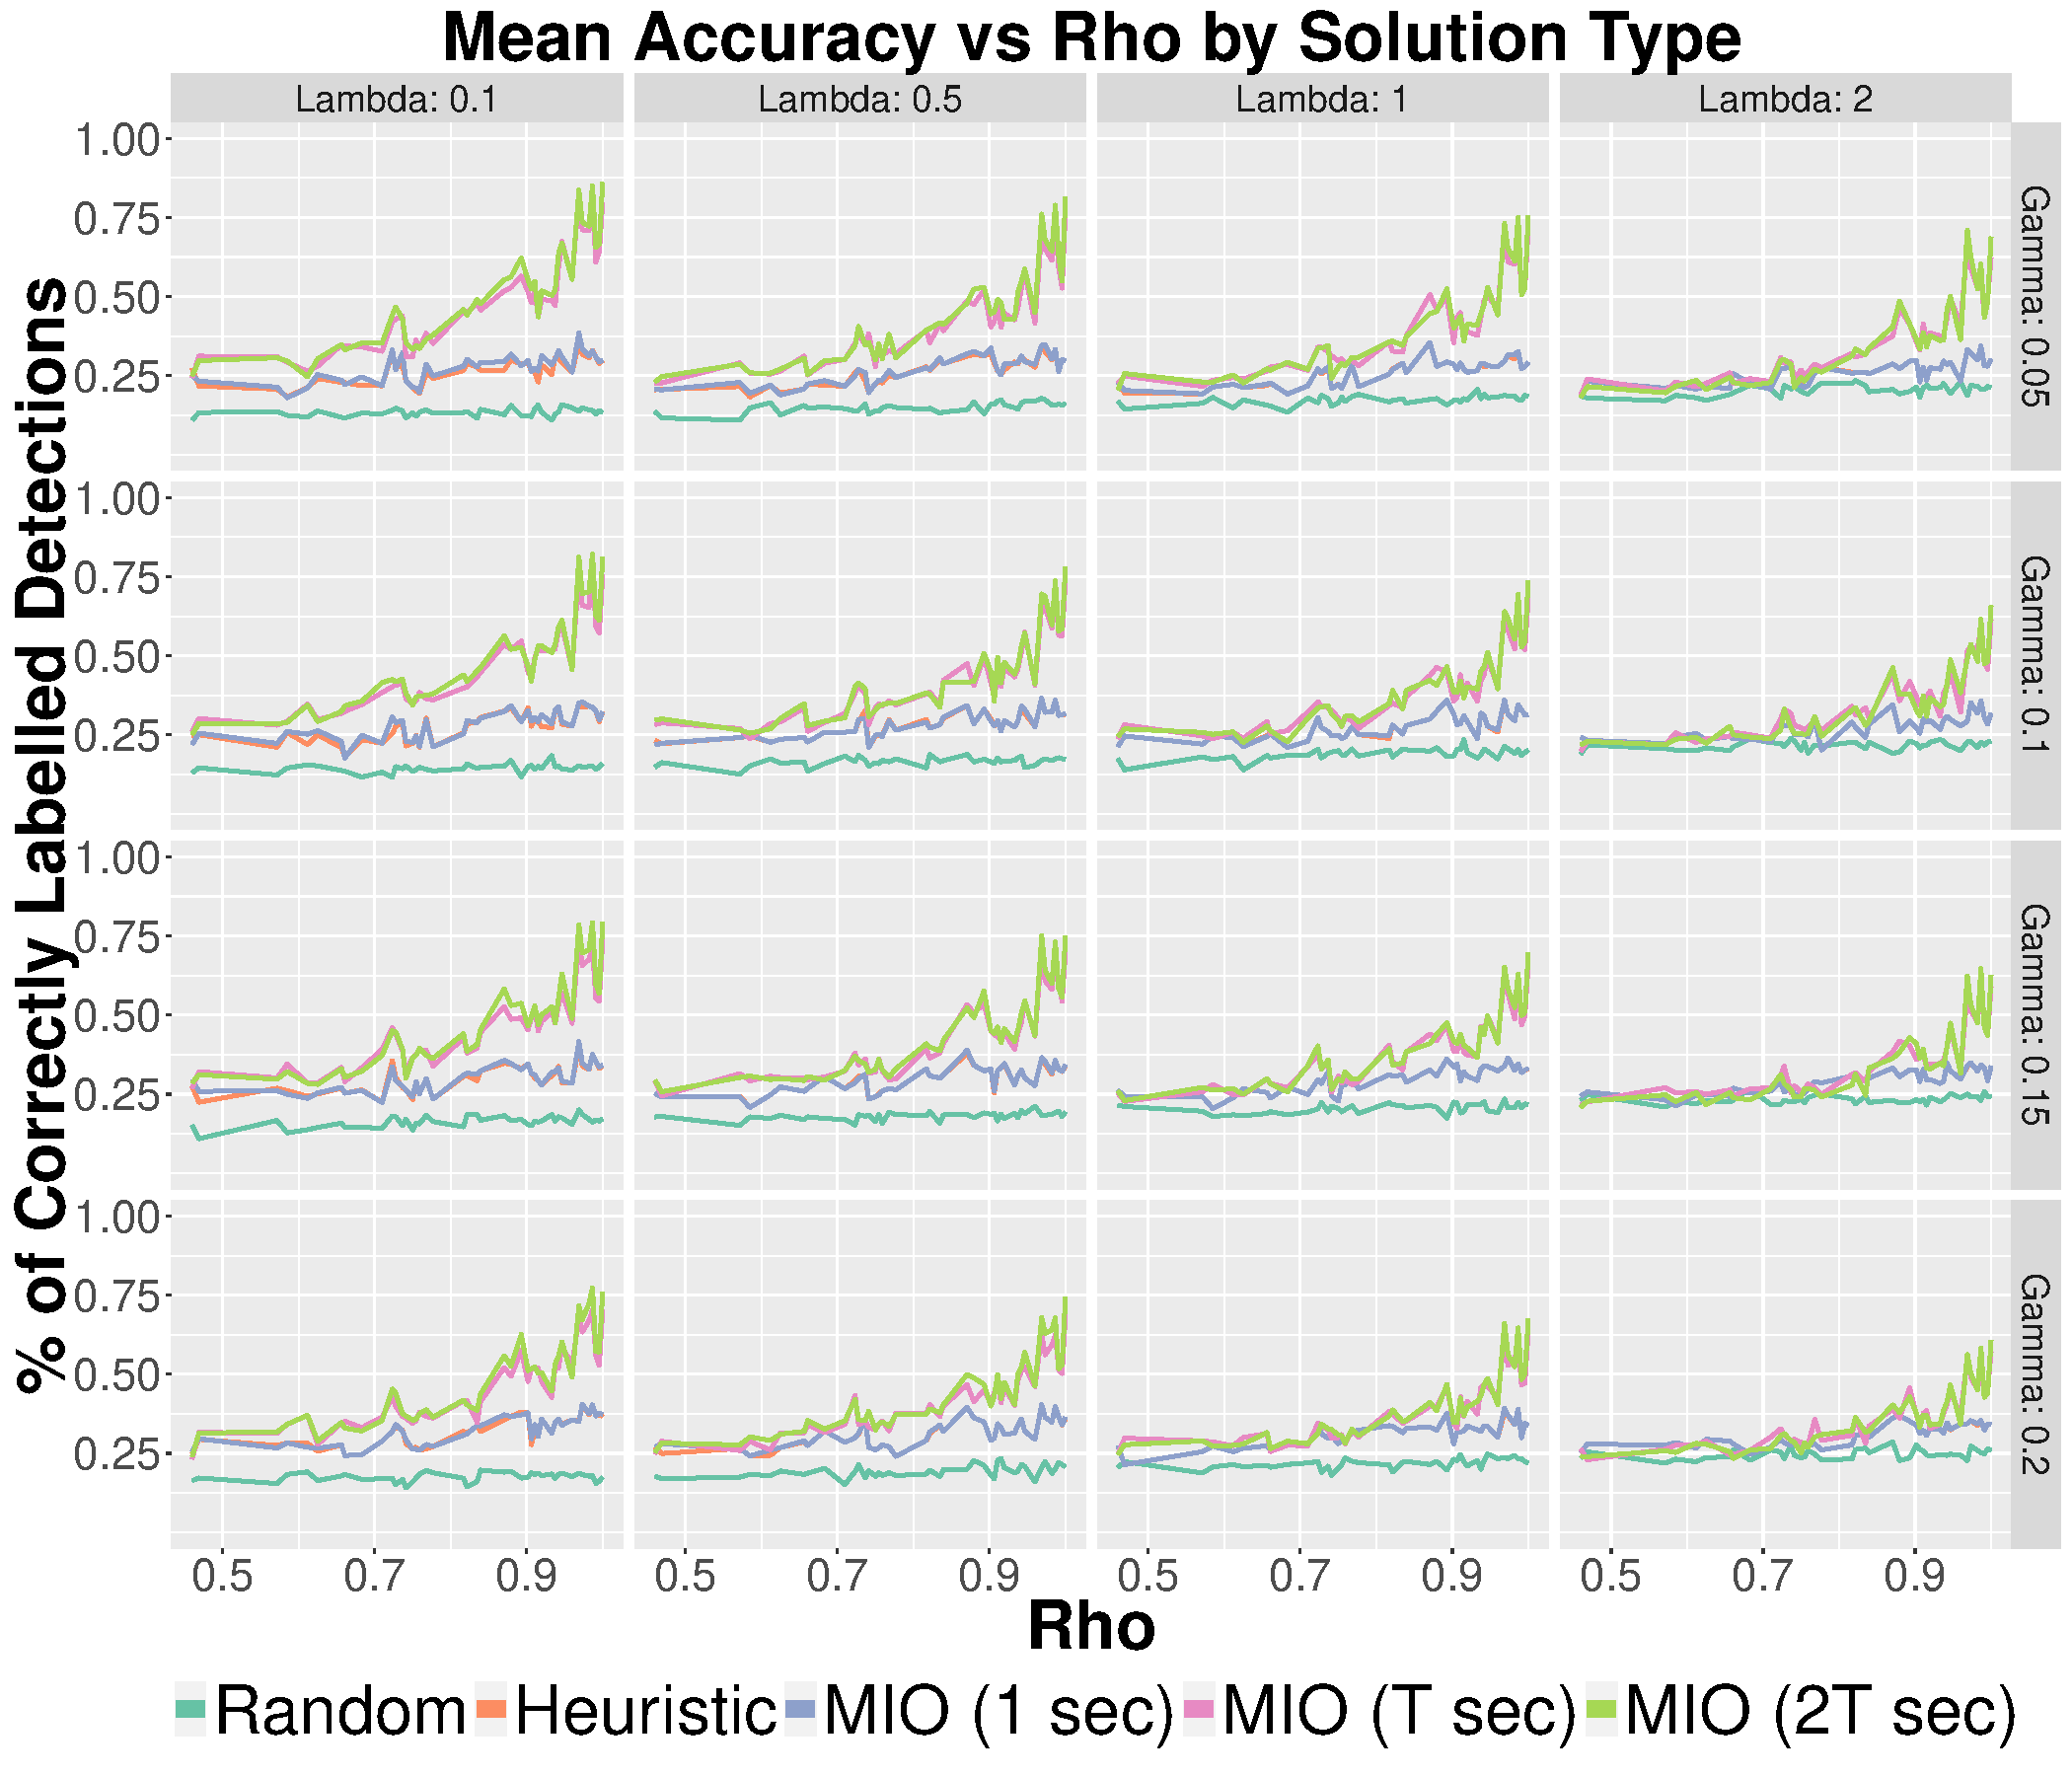
\includegraphics[width=\columnwidth]{../Figures/8_8_Accuracy}
  \caption{Accuracy of robust heuristic and MIO as compared to random solutions for scenarios of 8 targets and 8 scans, arranged by $\gamma$ and $\lambda$.}
  \label{fig:Robust_8_8_Accuracy}
\end{figure}

In Figure~\ref{fig:Robust_4_8_Accuracy} we see the accuracy results for four targets. In this case the heuristic solution is an significant improvement over the random solution, and is close to the best solution achieved by the MIO. The MIO achieves this best solution after 1 seconds, and no significant improvement is offered by running it for a longer period. In comparison, the accuracy in the eight targets scenarios, which is seen in Figure~\ref{fig:Robust_8_8_Accuracy}, the heuristic offers a smaller improvement to the random solution, and the MIO improves upon the heuristic solution only  after $T$ seconds, reaching its best accuracy. 

As we stated earlier, even with small values of $\lambda$ and $\gamma$ the case of detection ambiguity has an added difficulty of estimating the correct number of targets. Therefore, the fact that for $\lambda=0.1$ and $\gamma=0.05$ the decrease of accuracy with regard to the basic solution decreases by $5\%-10\%$ for both four and eight targets and across scenario difficulties suggests that we deal  well with this issue. Moreover, in the case of four target we reach a accuracy level above $90\%$  even for the highest value of $\gamma$ (where it was almost $100\%$ for the basic scenarios), suggesting that we are very close to the ideal association.

The robust approaches also appear to be more sensitive to higher false detection rates than higher missed detection probabilities. For example, for eight targets, fixing $\gamma=.05$, the MIO after $T$ accuracy decreases from about $90\%$ to $65\%$ when increasing $\lambda$ from $0.1$ to $2.0$, while fixing $\lambda=.1$ and increasing $\gamma$ from $.05$ to $.2$ reduces accuracy to $75\%$. This can also be attributed to our difficulty in tuning the penalties for higher levels of $\lambda$, which in turn, caused an over estimation of the number of targets, and therefore a reduced accuracy. 

\mysubsubsection{Trajectory Estimation}
We conclude our analysis of the robust approaches with a discussion on their performance in the sphere of the trajectory estimation problem. Figures~\ref{fig:Robust_4_8_Delta} and~\ref{fig:Robust_8_8_Delta} plot the $\delta$ performance metric against the detection error $\sigma$, for scenarios of four and eight targets, respectively. 
\begin{figure}[ht]
  \centering
  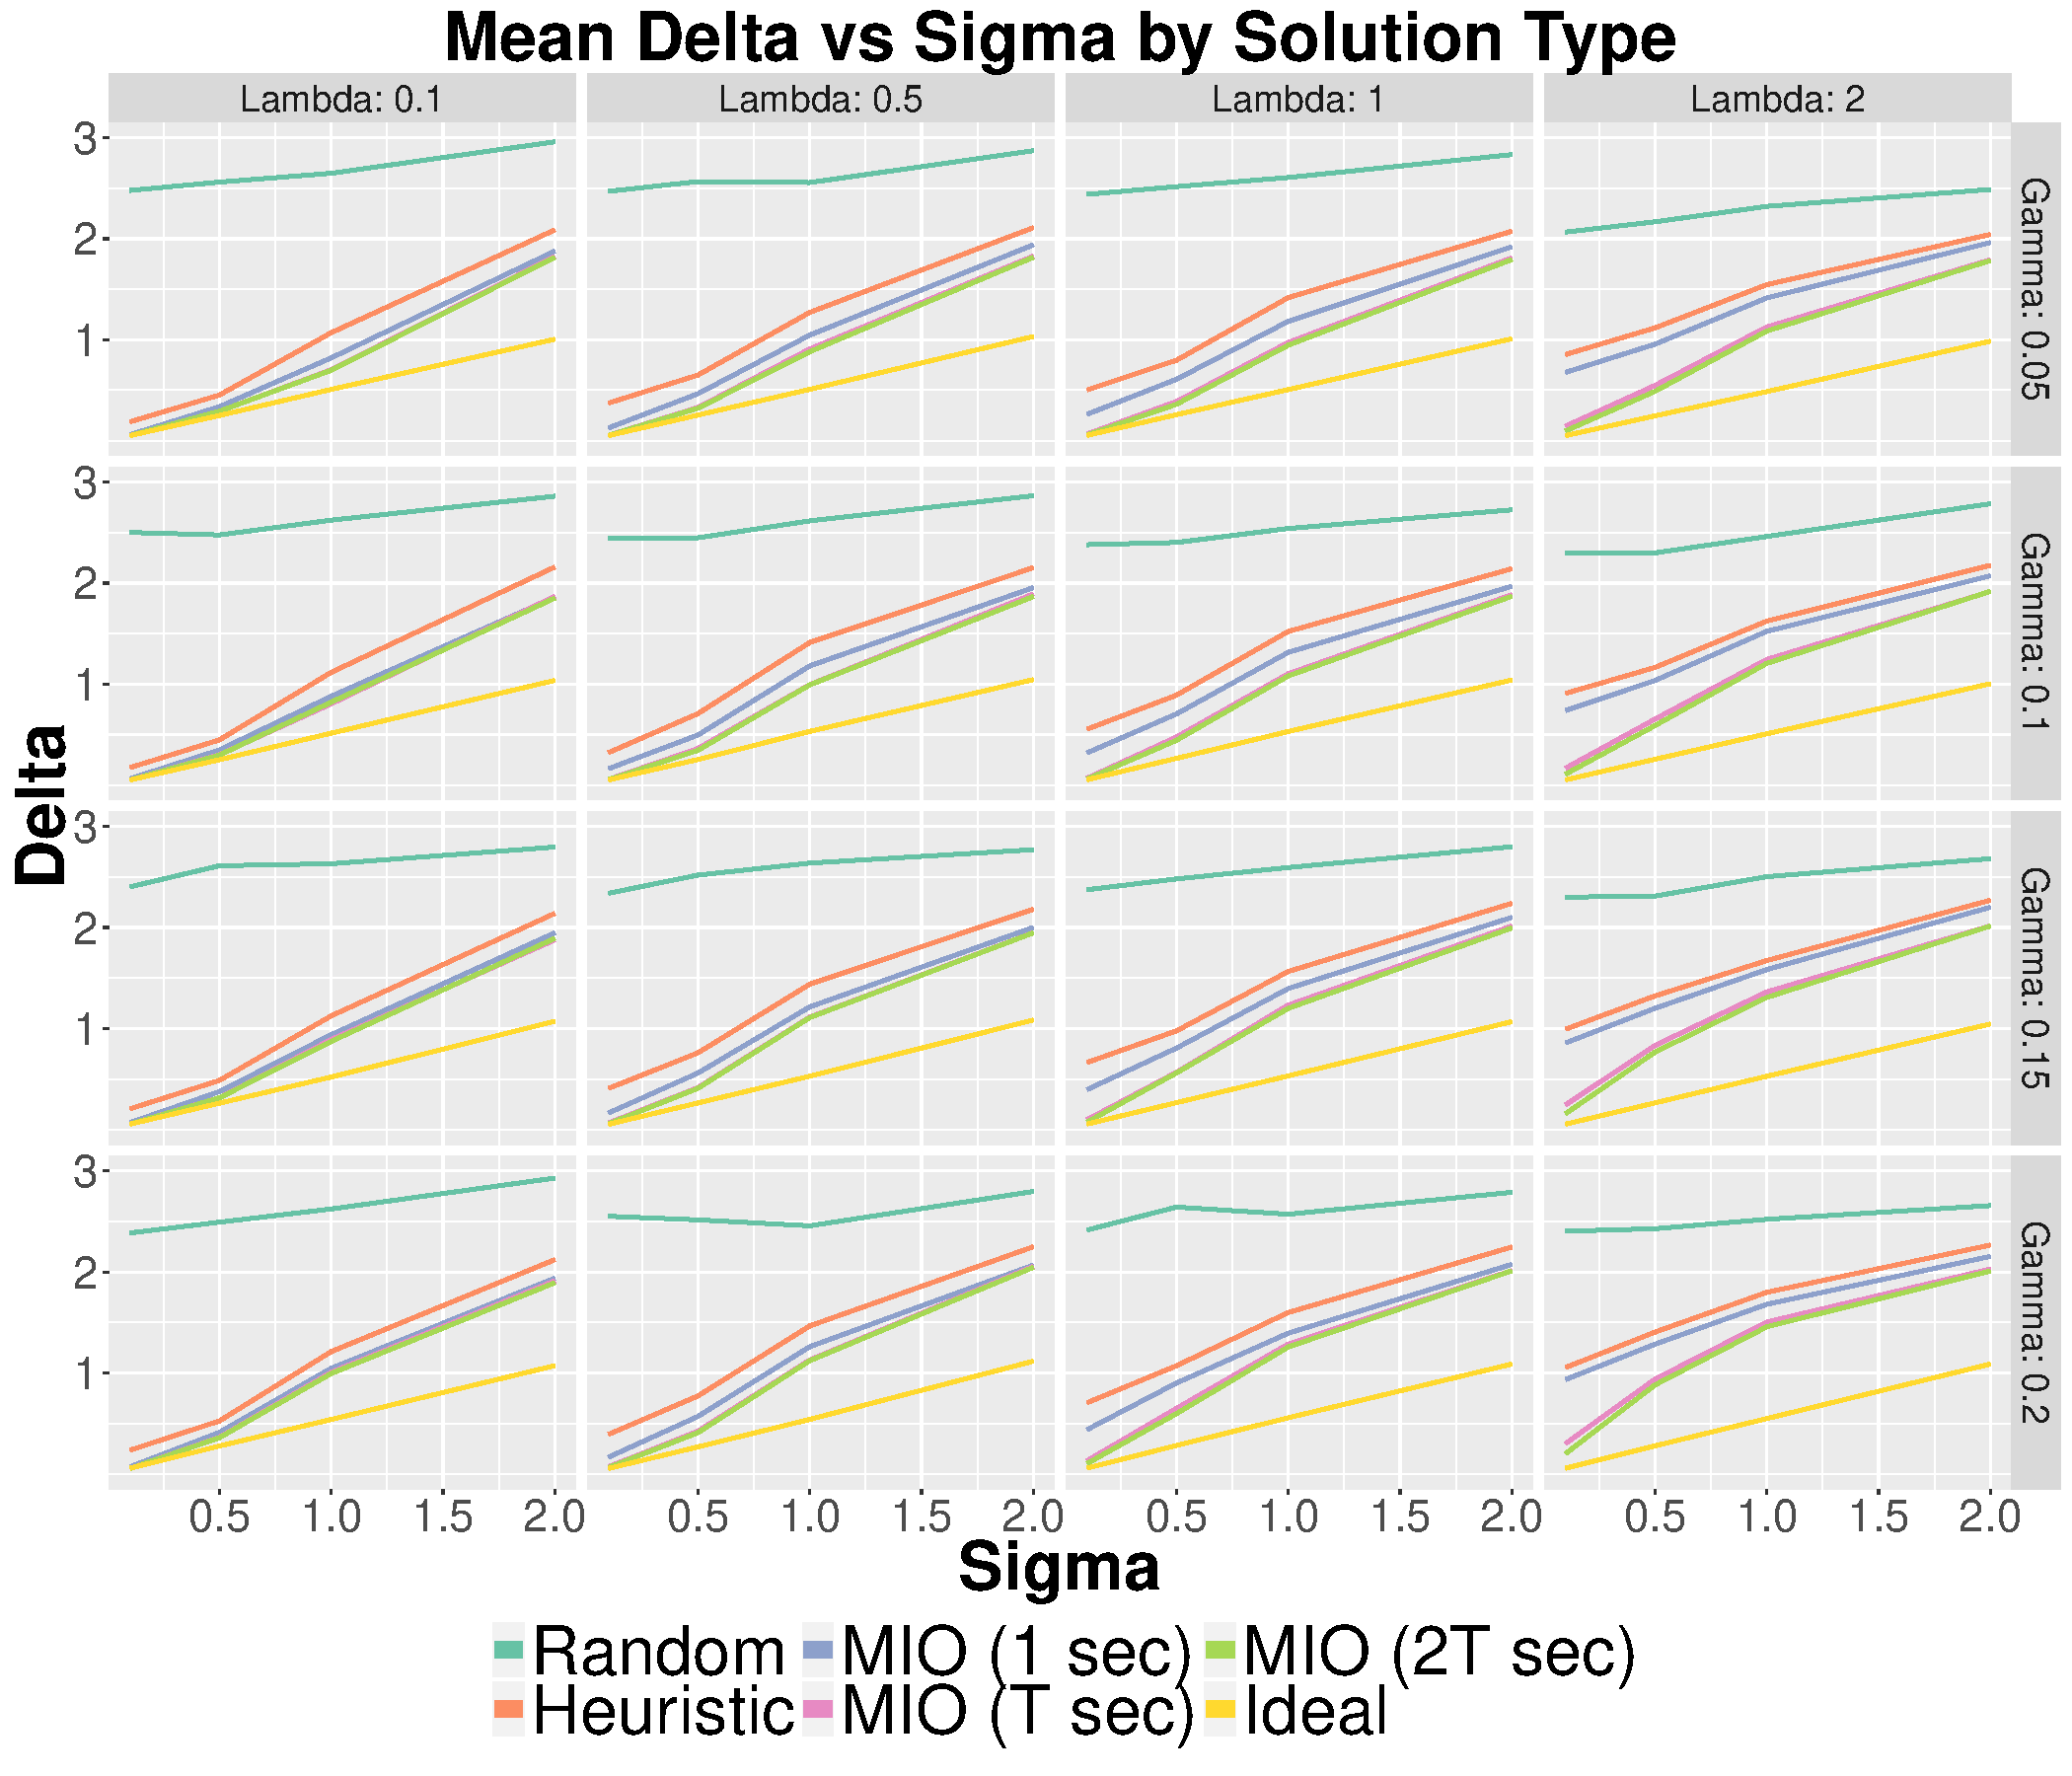
\includegraphics[width=\columnwidth]{../Figures/4_8_Delta}
  \caption{$\delta$ of robust heuristic and MIO as compared to random solutions for scenarios of 4 targets and 8 scans.}
  \label{fig:Robust_4_8_Delta}
\end{figure}
\begin{figure}[ht]
  \centering
  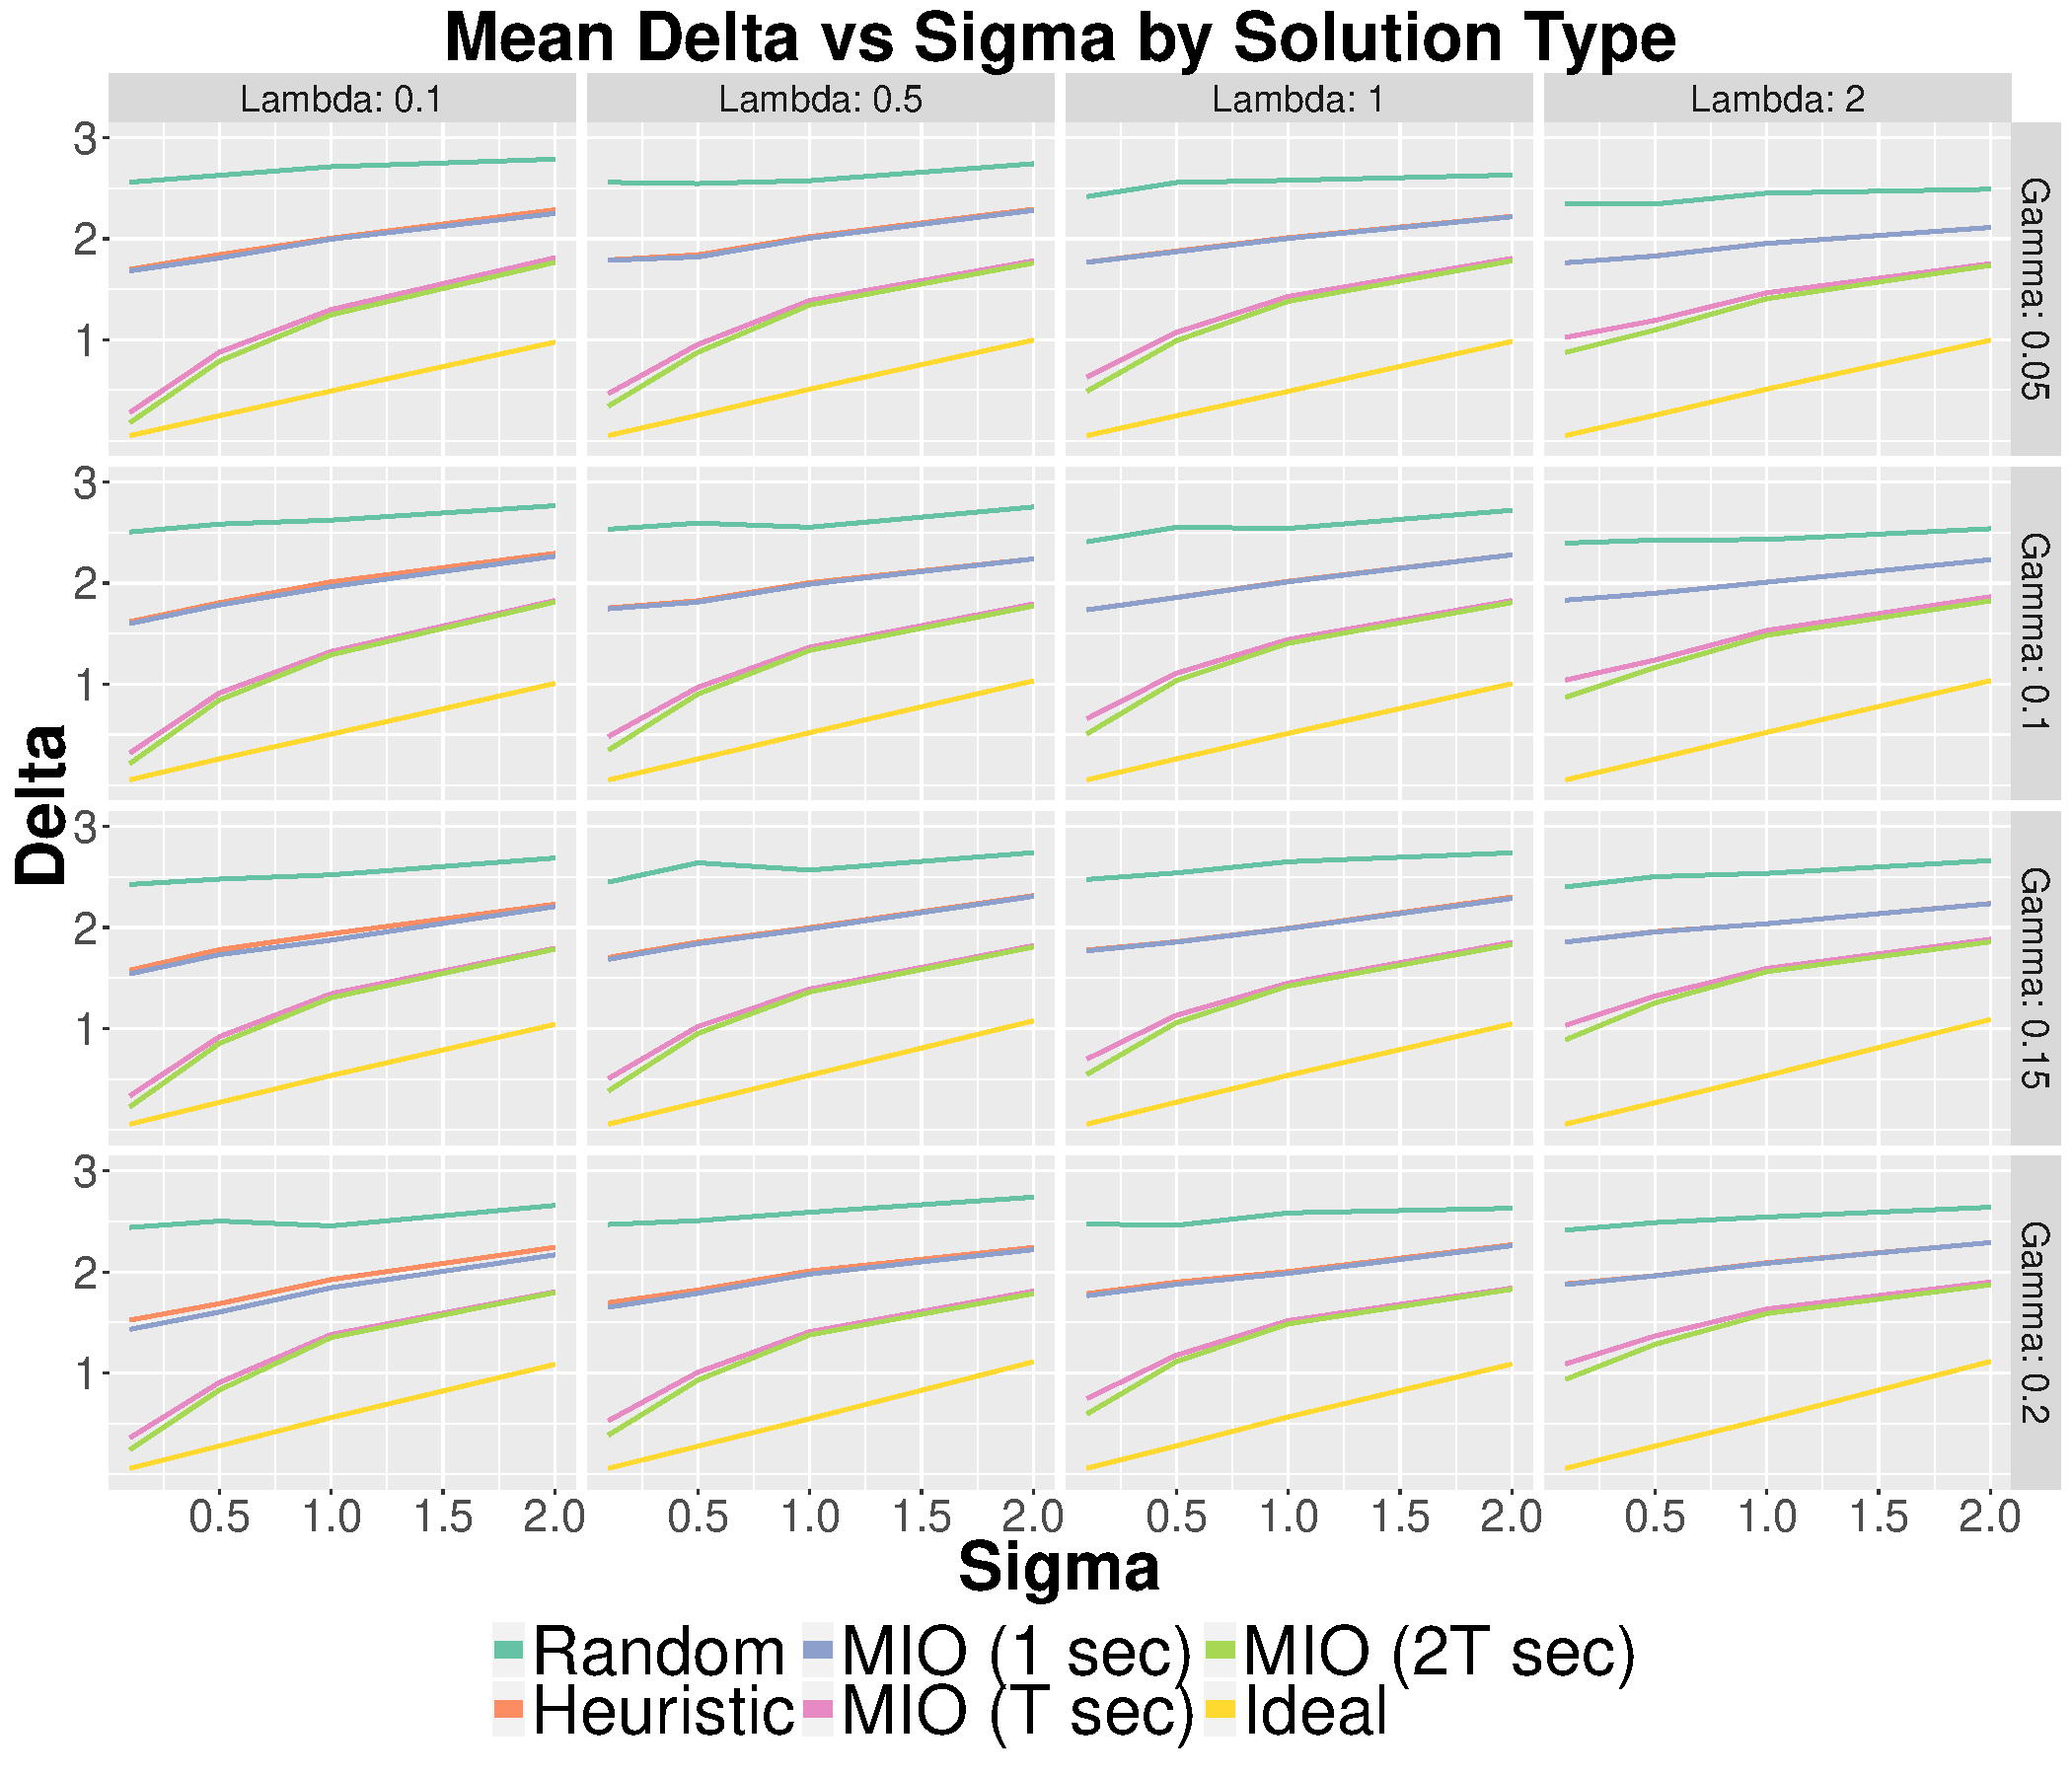
\includegraphics[width=\columnwidth]{../Figures/8_8_Delta}
  \caption{$\delta$ of robust heuristic and MIO as compared to random solutions for scenarios of 8 targets and 8 scans.}
  \label{fig:Robust_8_8_Delta}
\end{figure}

Note that $\delta$ is calculated using the $\min\{P_{\text{true}},P_{\text{est}}\}$. The fact that we tend to overestimate means that more often than not $\delta$ will be calculated using $P_{\text{true}}$. This implies that in most cases we match all the true trajectories to estimated ones, and so the number of trajectories for the $\delta$ calculation is the same as in the scenarios without detection ambiguity. Thus, we can compare and interpret their values directly.

In comparing Figure~\ref{fig:Robust_8_8_Delta} with the graph in Figure~\ref{Fig:Basic_Delta_Summary} corresponding to $P=8$ and $T=8$, we see that for $\lambda=0.1$ and $\gamma=0.05$ there is no observable loss of performance in adding the detection ambiguity, for the MIO after $T$ seconds. This observation also holds true for the heuristic solution. In contrast, comparing Figure~\ref{fig:Robust_4_8_Delta} with the graph in Figure~\ref{Fig:Basic_Delta_Summary} corresponding to $P=4$ and $T=8$, and the same $\lambda$ and $\gamma$ values, the $\delta$ value for the MIO increases for $\sigma$ values larger than $0.5$, and the increase becomes worse as $\sigma$ increases. Moreover, in the same case, the heuritic performance deteriorates even more sharply than the MIO's performance. 

Similar to what we have seen for the data association problem, in the trajectory estimation problem our approaches are also more robust to increases in $\gamma$ than increases in $\lambda$. Figures~\ref{fig:Robust_4_8_Delta} and~\ref{fig:Robust_8_8_Delta} both show that there is little to no loss in the quality of the trajectory estimation when increasing $\gamma$ for both the heuristic or MIO, and this holds true across all values of $\sigma$ and $\lambda$. Whereas, especially for small $\sigma$ values, as $\lambda$ increases we see the estimation of the MIO ran for $T$ seconds deteriorating, for example, for eight targets and $\sigma=0.1$, while for $\lambda=0.1$ we get $\delta$ close to zero, for $\lambda=2$ the value of delta increases to $1$.  This deterioration is a lot milder for the case of four targets.

\mysubsubsection{Detection Ambiguity Summary}
The case of detection ambiguity provides two additional challenges: the assignment problem is more complex for a fixed number of targets, and an added problem of deciding the correct number of target.
The results for this case indicate thats
\begin{itemize}
\item  Tuning the parameters leads to a correct estimation of the number of targets, even for a relatively large scenario.
\item The accuracy deteriorates by 5\%-10\% with the addition of detection ambiguity.
\item Although we tend to overestimate the number of targets, the quality of estimated trajectories that correspond to the true trajectories is similar to the case with no detection ambiguity.
\item The solution of the MIO is more robust to changes in missed detection probability than to changes in the false alarm rate.
\end{itemize}

\section{Summary and Future Work}\label{sec:Conclusion}
In this paper, we presented a new approach to the multi-target tracking problem which jointly solves the problems of data association and trajectory estimation via global optimization methods using a single objective function. Toward this goal, we proposed the use of a randomized local search heuristic as a warm start for a mixed integer optimization model, and we did so for scenarios with and without detection ambiguity. The approach is general since it makes no assumptions on the data generation process, and easily implementable, since it is based on a simple model with little to no tunable parameters. We showed that the local search heuristic finds good quality feasible solutions very quickly, and that the MIO offers improvement over the heuristic in seconds. We also show that while the introduction of detection ambiguity deteriorates the performance of the data association, it does not significantly effect the quality of trajectory estimation. Moreover, the quality of the solution obtained is robust to the missed detection rate, but less so to the false alarm rate.

The MIO and the heuristic runtimes are proportional to the number of scans and therefore, have limited scalability in that sense. However, they show potential for use in a sliding window scheme, which would use past decisions to fix detection assignments and thus add information for the current tracking window. This would allow us to track targets in real time systems for longer periods. 

Additionally, we observed that one of the key challenges in the case of detection ambiguity involves the correct estimation of the true number of targets. Our results suggest that tuning the penalties for a scenario with a certain number of targets may lead to over or underestimation for scenarios with a different number of targets. Therefore, we suggest additional research into more complex penalties that explore this dependency. 

Other areas for further research may lie in relaxing some of the scenario based assumptions, in particular, extensions to non-linear trajectories or the birth/death of targets. 

\appendices

\section{Detection Ambiguity Penalty Values}\label{app:Penalty_Appendix}
Here we provide recommendations for the tuning of penalty parameters $\theta$ and $\phi$. We begin with an explanation grounded in logic. It can be shown that as the false alarm rate $\lambda$ increases, the number of expected false alarms also increases. Therefore, it stands to reason that as a general rule of thumb the false alarm penalty $\theta$ should decrease as $\lambda$ increases. Similarly, the number of expected missed detections increases as the missed detection probability $\gamma$ increases, and so too the missed detection penalty $\phi$ should decrease. Furthermore, it stands to reason that the value of both of these penalties should somehow be tied to the value of $\sigma$, since in the objective function \eqref{eq: general_objective} there is a trade-off between the estimation error, which is tied to $\sigma$, and the penalties. Therefore, in order to balance this tradeoff, we should consider increasing both penalties as $\sigma$ increases. 

We also note that while in objective function \eqref{eq: general_objective} the total estimation error (the first term), as well as the number of missed detections (the third term) are proportional to the number of targets, the number of false alarms is independent of the number of targets. Since the number of target is unknown we can not tune the penalties to suit this number, and instead suggest that in order to balance the objective function terms we normalize $\theta$ for the number of targets the MIO is currently estimating. Towards this goal, we tune $\theta$ for scenarios with eight targets and use the following linear dependence to update $\theta(P_{\text{est}})$ for the estimated number of targets $P_{\text{est}}$:
$$\theta(P_{\text{est}})=\frac{P_{\text{est}}}{8}\theta.$$

Additionally, we empirically observed that the missed detection penalty $\phi$ benefits from tuning for the missed detection probability $\gamma$, the false alarm rate $\lambda$ and the detection error $\sigma$, while the false alarm penalty $\theta$  benefits from tuning for $\lambda$ and $\sigma$, but gains no added benefit from tuning for $\gamma$. %This may be explained by the fact that while the false alarm process is independent of the trajectory detection process, in the sense that it is not effected by a change in the number of trajectories, and so it only needs to balance the estimation errors which are proportional to $\sigma$, while deciding on whether to allow a missed detection is dependent on whether classifying a detection as a false alarm is plausible.

Through examination and experimentation we found these conclusions to generally hold true across a variety of scenario sizes and difficulties. Using the insight gained from these results, we tuned both penalties for the full scale experiment with detection ambiguity outlined in \mysection~\ref{\myabrv Results}. The false alarm penalties for the eight target scenarios in the robust experiment are shown in Table~\ref{tab:Theta_Penalties} and the missed detection penalties are shown in Table~\ref{tab:Phi_Penalties}.
\begin{table}[ht]
\centering
\begin{tabular}{c|m{1cm}m{1cm}m{1cm}m{1cm}}
  \hline
   & \multicolumn{4}{c}{$\sigma$} \\
   \cline{2-5}
   $\lambda$ & 0.1 & 0.5 & 1.0 & 2.0\\
  \hline
  \hline
   0.1 & 1.7 & 2.6 & 3.1 & 3.5 \\
   0.5 & 1.1 & 1.9 & 2.3 & 2.5 \\ 
   1.0 & 0.9 & 1.2 & 1.6 & 1.8 \\ 
   2.0 & 0.5 & 0.9 & 0.9 & 1.0 \\ 
   \hline
\end{tabular}
\caption{False alarm penalties ($\theta$) as a function of $\lambda$ and $\sigma$.}
\label{tab:Theta_Penalties}
\end{table}
\begin{table}[ht]
\centering
\begin{tabular}{cc|cccc}
  \hline
  & & \multicolumn{4}{c}{$\sigma$} \\
  \cline{3-6}
 $\lambda$ & $\gamma$ & 0.1 & 0.5 & 1 & 2 \\ 
  \hline
  \hline
   0.10 & 0.05 & 0.20 & 0.50 & 0.80 & 0.70 \\ 
   0.10 & 0.10 & 0.10 & 0.30 & 0.50 & 0.50 \\ 
   0.10 & 0.15 & 0.10 & 0.20 & 0.40 & 0.40 \\ 
   0.10 & 0.20 & 0.10 & 0.10 & 0.30 & 0.40 \\ 
   0.50 & 0.05 & 0.20 & 0.50 & 0.80 & 0.80 \\ 
   0.50 & 0.10 & 0.20 & 0.30 & 0.50 & 0.60 \\ 
   0.50 & 0.15 & 0.20 & 0.25 & 0.40 & 0.40 \\ 
   0.50 & 0.20 & 0.10 & 0.20 & 0.30 & 0.40 \\ 
   1.00 & 0.05 & 0.30 & 0.70 & 0.80 & 0.80 \\ 
   1.00 & 0.10 & 0.20 & 0.40 & 0.50 & 0.60 \\ 
   1.00 & 0.15 & 0.20 & 0.25 & 0.40 & 0.40 \\ 
   1.00 & 0.20 & 0.10 & 0.20 & 0.30 & 0.40 \\ 
   2.00 & 0.05 & 0.30 & 0.70 & 0.90 & 1.00 \\ 
   2.00 & 0.10 & 0.20 & 0.50 & 0.60 & 0.60 \\ 
   2.00 & 0.15 & 0.20 & 0.25 & 0.40 & 0.50 \\ 
   2.00 & 0.20 & 0.10 & 0.20 & 0.30 & 0.40 \\ 
   \hline
\end{tabular}
\caption{Missed detection penalties ($\phi$) as a function of $\lambda$, $\gamma$, and $\sigma$.}
\label{tab:Phi_Penalties}
\end{table}

\section{Robust MIO With Number of Targets as a Decision Variable}\label{app:Robust_Appendix}
\chapter{Figures}

\vspace*{-3in}

\begin{figure}
\vspace{2.4in}
\caption{Armadillo slaying lawyer.}
\label{arm:fig1}
\end{figure}
\clearpage
\newpage

\begin{figure}
\vspace{2.4in}
\caption{Armadillo eradicating national debt.}
\label{arm:fig2}
\end{figure}
\clearpage
\newpage


\section{Trajectory Assignment Pairing}\label{app:Assignment_Appendix}
In order to analyze the performance of a multi-target tracking algorithm, we must first find the best matching of the true trajectories of the scenario and the estimated trajectories of the algorithm solution. Put differently, we wish to find a set of assignment pairings which match true and estimated trajectories. Here we present a linear optimization model which solves for the globally optimal assignment pairings of true and estimated trajectories. In addition, we extend the assignment problem to scenarios with detection ambiguity, where the algorithm may overestimate or underestimate the number of targets. When this situation arises, a few minor adjustments are necessary to find the optimal assignment pairing. 

The goal of this assignment problem is to optimally assign pairs of true trajectories \textit{i} to estimated trajectories \textit{j} if there exists such a pairing to be made. Only a single set of decision variables are needed to determine if the true trajectory \textit{i} should be assigned to the estimated trajectory \textit{j} or not. 
\[y_{ij} = 
\begin{cases}
1, & \text{if true trajectory \textit{i} is assigned}\\
    & \text{ to estimated trajectory \textit{j},}\\
0, & \text{otherwise.}
\end{cases}\]

Remember that we denote the true position of trajectory \textit{i} at scan \textit{t} with $\bar{x}_{it}$ and the estimated position of trajectory \textit{j} at scan \textit{t} with $\hat{x}_{jt}$. Then the cost $c_{ij}$ of assigning true trajectory \textit{i} to estimated trajectory \textit{j} is the norm distance between these two trajectories as measured at each scan. 
\begin{align*}
	c_{ij} = \sum_{t=1}^{T} \|\bar{x}_{it} - \hat{x}_{jt}\|
\end{align*}
If we denote the true number of targets as $P_{\text{true}}$ and the estimated number of targets as $P_{\text{est}}$ then the objective of the integer optimization model would be:
\begin{align*}
\underset{y_{ij}}{\text{minimize: }} & \sum_{i=1}^{P_{\text{true}}} \sum_{j=1}^{P_{\text{est}}} c_{ij}y_{ij}
\end{align*}

When the number of true targets is equal to the number of estimated targets ($P_{\text{true}} = P_{\text{est}} = P$), we simply require two equality constraints to ensure that each true trajectory \textit{i} is assigned to exactly one estimated trajectory \textit{j} and vice versa. 
\begin{align}\label{eqn:assignment_1}
\sum_{i=1}^{P} y_{ij} = 1 \qquad \forall j = 1,...,P
\end{align}
\begin{align}\label{eqn:assignment_2}
\sum_{j=1}^{P} y_{ij} = 1 \qquad \forall i = 1,...,P
\end{align}

However, when the number of estimated trajectories differs from the number of true trajectories, these constraints must be modified slightly. In the case where the number of true targets exceeds the estimated number of targets ($P_{\text{true}}\geq P_{\text{est}}$), we restrict each true trajectory \textit{i} to the assignment of \textit{at most} one estimated trajectory \textit{j}, and Equation~\ref{eqn:assignment_1} is modified to:
\begin{align*}
\sum_{i=1}^{P_{\text{true}}} y_{ij} \leq 1 \qquad \forall  j = 1,...,P_{\text{est}}.
\end{align*}

On the contrary, when the number of estimated targets exceeds the true number of targets ($P_{\text{true}}\leq P_{\text{est}}$), then we restrict each estimated trajectory \textit{j} to the assignment of \textit{at most} one true trajectory \textit{i}, and Equation~\ref{eqn:assignment_2} is modified to:
\begin{align*}
\sum_{j=1}^{P_{\text{est}}} y_{ij} \leq 1 \qquad \forall i = 1,...,P_{\text{true}}.
\end{align*}

In summary, the generalized integer optimization assignment model is presented below.  
\begin{align*}
\underset{y_{ij}}{\text{minimize: }} & \sum_{i=1}^{P_{\text{true}}} \sum_{j=1}^{P_{\text{est}}} c_{ij}y_{ij}\\
\text{subject to: }	& \sum_{i=1}^{P_{\text{true}}} y_{ij} = 1 \qquad \forall j = 1,...,P_{\text{est}} \nonumber \\
				& \sum_{j=1}^{P_{\text{est}}} y_{ij} = 1 \qquad \forall i = 1,...,P_{\text{true}} \nonumber \\
				& y_{ij} \in \{0,1\} \quad \forall i = 1,...,P_{\text{true}},j = 1,...,P_{\text{est}} \nonumber
\end{align*}
This model is vital to scoring the performance of an MTT algorithm's solution because it ensures the globally optimal pairing of true and estimated trajectories.




\section*{Acknowledgments}
The authors would like to thank Sung-Hyun Son, Ph.D. and Steven Relyea at Lincoln Laboratories for introducing us to the MTT problem and for their ongoing guidance throughout this work. Additionally, we would like to thank Lincoln Laboratories and the LLGrid team for their continual support in running our experiments. 

This material is based upon work supported by the Air Force under Air Force Contract No. FA8721-05-C-0002 and/or FA8702-15-D-0001. The views expressed in this document are those of the authors and do not reflect the official policy or position of the United States Air Force, the United States Department of Defense or the United States Government.

%\IEEEtriggeratref{15}
% The "triggered" command can be changed if desired:
%\IEEEtriggercmd{\enlargethispage{-5in}}


\bibliographystyle{IEEEtran}
\bibliography{Bibliography}

\end{document}